%\documentclass[12pt,a4paper]{article}
\documentclass[12pt,a4paper]{scrartcl}
%\documentclass[11pt,a4paper,oneside]{book}
% ===================== PACKAGES =====================
\usepackage[british]{babel}
\usepackage[tmargin=1in, bmargin=1in, lmargin=0.75in, rmargin=0.75in]{geometry}
\usepackage[dvipsnames,table]{xcolor}  % prima di tikz, listings, ecc.

\usepackage{tikz}
\usepackage{graphicx}
\usepackage{pgfplots}
\pgfplotsset{width=12cm, compat=1.9}
\usepackage{setspace}
\usepackage{chemmacros}
\usepackage{chemfig}
\usepackage{esint}
\usepackage{tabularray}
\usepackage{makeidx}
\usepackage{epstopdf}
\usepackage{amssymb}
\usepackage{mathrsfs}
\usepackage{bm}
\usepackage{amsmath}
\usepackage{enumitem}
\usepackage[english]{varioref}
\usepackage{lipsum}
\usepackage{fancyhdr}
\usepackage{float}
\usepackage{empheq}
\usepackage[framemethod=tikz]{mdframed}
\numberwithin{equation}{section}
\usepackage{eso-pic}
\usepackage{calc}
\usepackage{nccmath}
\usepackage{caption}
\usepackage{subcaption}
\usepackage{gensymb}
\usepackage{amsfonts, amsthm, epsfig, epstopdf, titling, url, array}
\usepackage{tabularx}
\usepackage{makecell}
\usepackage{booktabs}
\usepackage{array}
\usepackage{siunitx}
\sisetup{input-digits=0123456789\pi}
\usepackage[symbol]{footmisc}
\usepackage{multicol}
\usepackage{boondox-cal}
\usepackage{blindtext}
\usepackage{changepage}
\usepackage{nomencl}
\usepackage{hyperref}
\usepackage{xurl}
\usepackage{ragged2e}
\usepackage[version=4]{mhchem}  % ← conflitto di opzioni
\usepackage{longtable}
\usepackage{chemformula}
\usetikzlibrary{arrows.meta,positioning,calc}

% ===================== SI UNITS =====================
\DeclareSIUnit\atm{atm}
\DeclareSIUnit{\var}{var}
\DeclareSIUnit{\pu}{p.u.}


% ===================== MATH OPERATORS =====================
\DeclareMathOperator{\rank}{rank}
\DeclareMathOperator{\atantwo}{atan2}
\DeclareMathOperator{\spn}{span}

% ===================== COMMANDS =====================
\newcommand{\abs}[1]{\left|#1\right|}
\newcommand{\sign}{\text{sign}}
\newcommand{\centered}[1]{\begin{tabular}{@{}l@{}} #1 \end{tabular}}

% ===================== COLORS =====================
\definecolor{mycolor1}{rgb}{0.97, 0.97, 0.97}
\definecolor{mycolor2}{rgb}{0.97, 0.97, 0.97}
\definecolor{tableShade}{gray}{0.9}

% ===================== THEOREM ENVIRONMENTS =====================
\theoremstyle{it}
\newtheorem{defn}{Definition}[section]
\newtheorem{assumption}{Assumption}[section]
\newtheorem{thm}{Theorem}[section]
\newtheorem{lemma}{Lemma}[section]
\newtheorem{corollary}{Corollary}[section]
\theoremstyle{definition}
\newtheorem{example}{Example}[section]

% ===================== CUSTOM ENVIRONMENTS =====================
\newenvironment{myitemize_1}{
	\begin{itemize}[topsep=0pt]
		\setlength{\topsep}{2pt}
		\setlength{\itemsep}{2pt}
		\setlength{\parskip}{2pt}
		\setlength{\parsep}{2pt}
	}{\end{itemize}}

\newmdenv[
innerlinewidth=0.5pt,
roundcorner=4pt,
backgroundcolor=mycolor2,
linecolor=mycolor1,
innerleftmargin=6pt,
innerrightmargin=6pt,
innertopmargin=6pt,
innerbottommargin=6pt
]{mybox}

% ===================== TABLE COLUMN TYPES =====================
\newcolumntype{Y}{>{\hsize=2\hsize}X}
\newcolumntype{Z}{>{\centering\arraybackslash\hsize=0.857\hsize}X}

% ===================== SECTION DEPTH =====================
\setcounter{secnumdepth}{3}
\setcounter{tocdepth}{3}

% ===================== PAGE STYLE =====================
\setlength{\headheight}{20pt}
\setlength{\headsep}{20pt}

\pagestyle{fancy}
\fancypagestyle{firstpage}{\rhead{}}
\fancyhead[L]{\slshape\nouppercase{\leftmark}}
\chead{}
\rhead{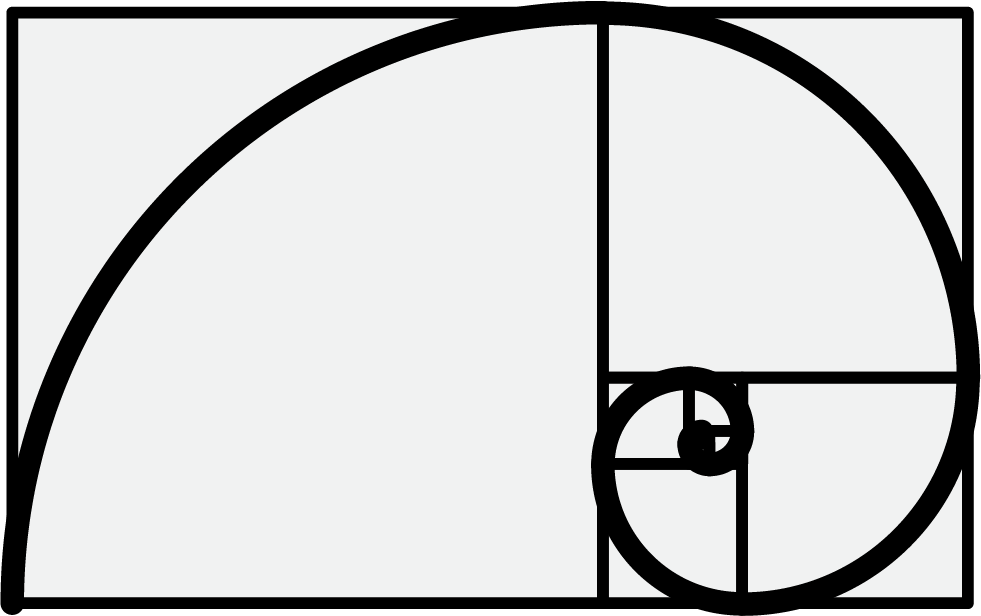
\includegraphics[height=0.75cm]{../../AAA_template_latex_settings/pwr-control_logo_doc.png}}
\lfoot{\href{http://www.pwr-control.com}{pwr-control.com}}
\cfoot{-\ \thepage\ -}
\rfoot{\textit{}}
\renewcommand{\headrulewidth}{0.4pt}
\renewcommand{\footrulewidth}{0.4pt}


\geometry{
	a4paper,
	top    = 2.5cm,
	bottom = 3.0cm,
	left   = 2.5cm,
	right  = 2.5cm
}

\hypersetup{
	colorlinks = true,
	urlcolor   = blue,
	linkcolor  = black,
	citecolor  = black
}

\pagenumbering{gobble}
\setlength{\emergencystretch}{3em}
%\newcommand{\ohm}{\,\Omega}
\newcommand{\ud}{\,\mathrm{d}}
\newcommand{\Zmat}{\bm{Z}}
\newcommand{\Ymat}{\bm{Y}}
\newcommand{\Rmat}{\bm{R}}
\newcommand{\Lmat}{\bm{L}}
\newcommand{\Cmat}{\bm{C}}
\newcommand{\Gmat}{\bm{G}}
\newcommand{\Vvec}{\bm{V}}
\newcommand{\Ivec}{\bm{I}}

% =============================================================
%  
% =============================================================

\newcommand{\DocCategory}{Technical Research Report}
\newcommand{\DocField}{Power Electronics and Control Systems}

\newcommand{\DocTitle}{%
	{\fontsize{20}{24}\selectfont\bfseries PS-12V-12kA:} \\[16pt]
	{\fontsize{16}{20}\selectfont\bfseries power supply for electrolysis.}
}

\newcommand{\DocSubtitle}{%
	Dimensioning of power supply for electrolysis application. 
}

\newcommand{\DocAuthor}{Davide Bagnara}
\newcommand{\DocDate}{July 2026}

\newcommand{\DocAbstract}{%
	This report presents the design and simulation-based verification of a 300 kW power supply unit for electrolysis applications, rated 25 V / 12 kA at nominal load and supplied from a three-phase 480 V grid. The proposed architecture comprises two conversion stages: a grid-tied Active Front End (AFE) rectifier interfaced through an LCL filter exploiting the point-of-common-coupling inductance, and an isolated Phase-Shift Full Bridge Converter (PS-FBC) with center-tapped high-frequency transformers and a high-current diode rectifier stage. The design addresses the stringent requirements of galvanic isolation, output voltage ripple below 0.25 V rms, grid current distortion $\text{THD}_i<5\% $, and power factor above 0.95 over the entire operating range. Component sizing — including the LCL filter, DC-link capacitor banks, HF transformer series inductance enabling Zero-Voltage Switching, and welding-grade rectifier diodes — is reported together with a complete loss budget, yielding an estimated overall efficiency of approximately $91.7\%$, in compliance with the $\eta > 90 \%$ specification. The full AFE + PS-FBC system, based on CM1200DW-24T LV100 IGBT modules, is validated in MATLAB/Simulink/Simscape under two operating scenarios, nominal load cold (NLC, 25 V / 12 kA) and nominal load hot (NLH, 10 V / 12 kA), reporting voltages, currents and power losses of the main active and passive components.
}


% Tre righe metadati in fondo (label small caps + valore)
\newcommand{\MetaLabelA}{Project Repository}
\newcommand{\MetaValueA}{https://github.com/pwr-control/modelization-and-control.git}
\newcommand{\MetaValueAUrl}{https://github.com/pwr-control/modelization-and-control.git}
\newcommand{\MetaValueALabel}{modelization-and-control.git}


\newcommand{\MetaLabelB}{Framework}
\newcommand{\MetaValueB}{MATLAB/Simulink/Simscape}

\newcommand{\MetaLabelC}{Architecture}
\newcommand{\MetaValueC}{SiC, EiceDRIVER, Customized Power Supplies}

% =============================================================
%  FRONTESPIZIO
% =============================================================
\begin{document}
	\titlepage
	% ---- Intestazione centrata ----
	\begin{center}
		{\Large\scshape \DocCategory}\\[8pt]
		{\large\scshape \DocField}
	\end{center}
	
	\vspace{36pt}
	\noindent\rule{\linewidth}{0.8pt}
	
	% ---- Titolo ----
	\vspace{16pt}
	\begin{center}
		\DocTitle
	\end{center}
	
	\vspace{4pt}
	\noindent\rule{\linewidth}{2.2pt}
	
	% ---- Sottotitolo ----
	%\vspace{14pt}
	\begin{center}
		\begin{onehalfspace}
			{\large\itshape \DocSubtitle}
		\end{onehalfspace}
	\end{center}
	
	% ---- Spazio prima di Autore/Data ----
	\vspace{18pt}
	
	% ---- Author / Date su due colonne ----
	\begin{minipage}{0.92\linewidth}
		\noindent
		\begin{minipage}[t]{0.48\linewidth}
			\textbf{Author:}\\[2pt]
			\DocAuthor
		\end{minipage}%
		\hfill
		\begin{minipage}[t]{0.48\linewidth}
			\raggedleft
			\textbf{Date:}\\[2pt]
			\DocDate
		\end{minipage}
	\end{minipage}
	% ---- Spazio prima dell'abstract ----
	\vspace{36pt}
	
	% ---- Abstract indentato ----
	\begin{center}
		\begin{minipage}{0.85\linewidth}
			%    \small
			\footnotesize 
			\begin{onehalfspace}
				\textbf{Abstract:} \DocAbstract
			\end{onehalfspace}
		\end{minipage}
	\end{center}
	
	% ---- Spazio prima dei metadati ----
	\vfill
	
	% ---- Metadati in fondo ----
	\noindent
	\begin{tabular}{@{} r @{\quad} l @{}}
		%		\textsc{\MetaLabelA:} & {\url{\MetaValueA}} \\[3pt]
		\textsc{\MetaLabelA:} & {\href{\MetaValueAUrl}{\MetaValueALabel}} \\[3pt]
		\textsc{\MetaLabelB:} & {\MetaValueB}       \\[3pt]
		%		\textsc{\small\MetaLabelC:} & {\small\MetaValueC}       \\
	\end{tabular}
	
	% =============================================================
	%  Fine frontespizio
	% =============================================================
	\newpage
	\pagenumbering{arabic}
	\setcounter{page}{1}
	\tableofcontents
	\listoffigures	
	\listoftables
	\newpage
	
\section*{Nomenclature}
\begin{itemize}
	\item[--] AFE: active front end;
	\item[--] HF-TR: high-frequency transformer;
	\item[--] PS-FBC: phase-shift full bridge converter;
	\item[--] LCL: inductor-capacitor-inductor filter;
	\item[--] $\text{THD}_\text{i}$: current total harmonic distortion;
	\item[--] $L_\text{grid}\quad\Big[\SI{}{\henry}\Big]$: point of common coupling ({PCC}) inductance and \emph{LCL} output filter inductance;
	\item[--] $C_\text{Fu}\quad\Big[\SI{}{\farad}\Big]$: \emph{LCL} output filter capacitor;	
	\item[--] $R_\text{CFu}\quad\Big[\SI{}{\ohm}\Big]$: damping of the LCL output filter capacitor;	
	\item[--] $L_\text{Fu}\quad\Big[\SI{}{\henry}\Big]$: \emph{LCL} input filter inductance;	
	\item[--] $C_\text{Fi}\quad\Big[\SI{}{\farad}\Big]$: dclink capacitor of the AFE stage;	
	\item[--] $C_\text{dc}^{dc1}\quad\Big[\SI{}{\farad}\Big]$: input capacitor of the PS-FBC stage;	
	\item[--] $C_\text{dc}^{dc2}\quad\Big[\SI{}{\farad}\Big]$: output capacitor of the PS-FBC stage;	
	\item[--] $L_\text{dc}^{dc2}\quad\Big[\SI{}{\henry}\Big]$: output inductance of the PS-FBC stage;
	\item[--] $L_\text{s}\quad\Big[\SI{}{\henry}\Big]$: series inductance of the PS-FBC stage;	
	\item[--] $\vec{u}_\text{g}^\text{abc}(t)\quad\Big[\SI{}{\volt}\Big]$: grid voltage used by AFE for PLL grid synchronization;	
	\item[--] $\vec{i}_\text{g}^\text{abc}(t)\quad\Big[\SI{}{\ampere}\Big]$: grid current used for PF and $\text{THD}_\text{i}$ evaluation;	
	\item[--] $u_\text{dc}^\text{dc1}(t)\quad\Big[\SI{}{\volt}\Big]$: AFE stage dclink voltage;	
	\item[--] $u_\text{ac}^\text{ac1}(t)\quad\Big[\SI{}{\volt}\Big]$: transformer input voltage;			
	\item[--] $i_\text{ac}^\text{ac1}(t)\quad\Big[\SI{}{\ampere}\Big]$: transformer input current;		
	\item[--] $i_\text{d}^\text{dn}(t)\quad\Big[\SI{}{\ampere}\Big]$: n-th diode rectifier current;	
	\item[--] $f_\text{pwm}^\text{afe}\quad\Big[\SI{}{\hertz}\Big]$: AFE switching frequency;
	\item[--] $f_\text{pwm}^\text{fbc}\quad\Big[\SI{}{\hertz}\Big]$: PS-FBC switching frequency.		
\end{itemize}
\begin{onehalfspace}
\section{Introduction}

The system described in this document is designed to deliver a nominal output voltage of \SI{25}{\volt} at \SI{12}{\kilo\ampere},
corresponding to a rated power of \SI{300}{\kilo\watt}, from a three-phase \SI{480}{\volt} mains supply.

The document is structured as follows. Section~\ref{sec:specs} summarises the electrical
and thermal specifications together with the two operating conditions defined for
compliance verification: nominal load cold (\textbf{NLC}) and nominal load hot (\textbf{NLH}).
Section~\ref{sec:topology} presents the selected topology and justifies the design choices
with respect to efficiency, current ripple, and controllability.
The converter design — including transformer architecture, switching-stage sizing, and
output filter — is detailed in Section~\ref{sec:design}. Simulation results are shown in Section~\ref{sec:sim}.

\section{Power Supply Specification}\label{sec:specs}
In this section a list of requirements and constraints which the power supply shall satisfy is reported. 

\begin{itemize}
	\item[--] Overall performance and requirements:
	\begin{itemize}
		\item[--] Nominal Output Voltage, $V_\mathrm{out}^\mathrm{nom} = \SI{25}{\volt}$.
		\item[--] Nominal Output Current, $I_\mathrm{out}^\mathrm{nom} = \SI{12}{\kilo\ampere}$.
		\item[--] Nominal Output Power, $P_\mathrm{out}^\mathrm{nom} = \SI{300}{\kilo\watt}$.
		\item[--] Maximum Output Voltage Ripple, $\Delta v_\mathrm{out} \le \SI{0.25}{\volt}$ (rms).
		\item[--] Current accuracy, $\lvert\tilde{i}\rvert_\mathrm{max} \le \SI{1}{\percent}$.
		\item[--] Voltage accuracy, $\lvert\tilde{v}\rvert_\mathrm{max} \le \SI{0.5}{\percent}$.
		\item[--] Efficiency, $\eta > \SI{90}{\percent}$.
		\item[--] The power supply shall provide galvanic isolation.
		\item[--] Maximum grid current distortion, $\mathrm{THD}_i < \SI{5}{\percent}$.
		\item[--] Power Factor, $\mathrm{PF} > \num{0.95}$ over the entire operating range.
	\end{itemize}
	\item[--] Electrical power source specifications:
	\begin{itemize}
		\item[--] Grid Voltage, $V_\mathrm{grid} = \SI{480}{\volt}$,
		operative range \SI[retain-explicit-plus]{+5}{\percent}~/~\SI{-10}{\percent}.
		\item[--] Grid Frequency, $f_\mathrm{grid} = \SI{50}{\hertz}$ / \SI{60}{\hertz},
		$\pm\SI{2}{\percent}$.
		\item[--] Short-Circuit Current at PCC, $I_\mathrm{cc} = \SI{15}{\kilo\ampere}$.
	\end{itemize}
	\item[--] Liquid cooled (de-ionized water not specified).
	\item[--] Operative working condition as shown in Figure~\ref{current_profile}.
\end{itemize}

\begin{figure}[H]
	\centering
	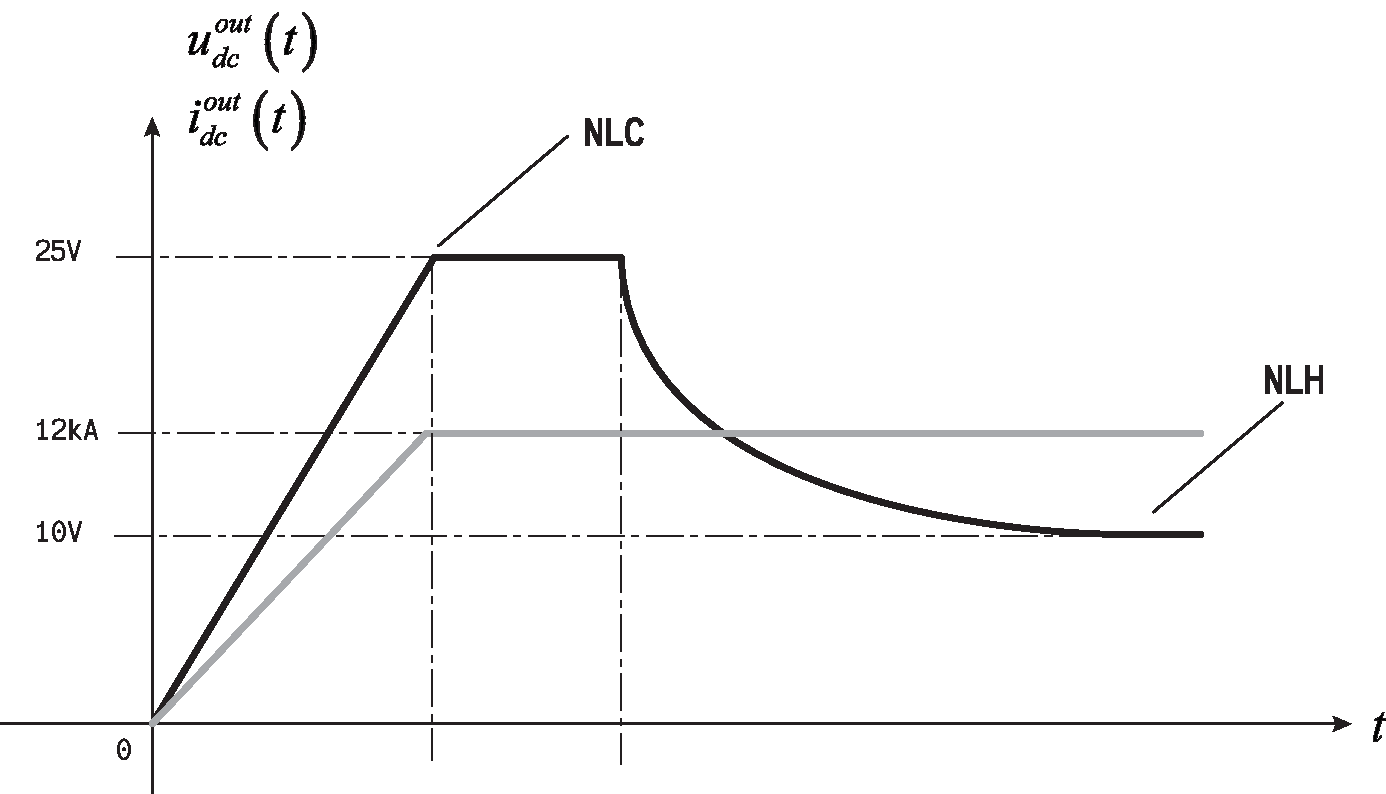
\includegraphics[width = 375pt, 
	keepaspectratio]{figures/current_profile.pdf}
	\captionsetup{width=.75\textwidth}
	\caption{Load current and voltage profile under different operative conditions (NLC and NLH).}
	\label{current_profile} 
\end{figure}

\section{Power Supply Architecture}\label{sec:design}
The demanding nature of this specification — in particular the combination of very high
output current, tight ripple and regulation requirements, and the need for galvanic
isolation — calls for a carefully selected power conversion architecture. The proposed solution consists of two power conversion stages:
\begin{itemize}
	\item[--] an Active Front End (AFE) rectifier;
	\item[--] an isolated DC/DC converter based on a Full Bridge Converter (here called PS-FBC, where PS stands for phase-shifted).
\end{itemize}
As set out in the specifications above, satisfying the requirements of
unity-adjacent power factor ($\mathrm{PF} > 0.95$), low grid current
distortion ($\mathrm{THD}_i < 5\%$), and galvanic isolation calls for the
two-stage solution described hereafter, comprising an AFE stage
(see Figure~\ref{fig:afe}) and a PS-FBC stage (see Figure~\ref{fig:psfbc}).

\begin{figure}[H]
	\centering
	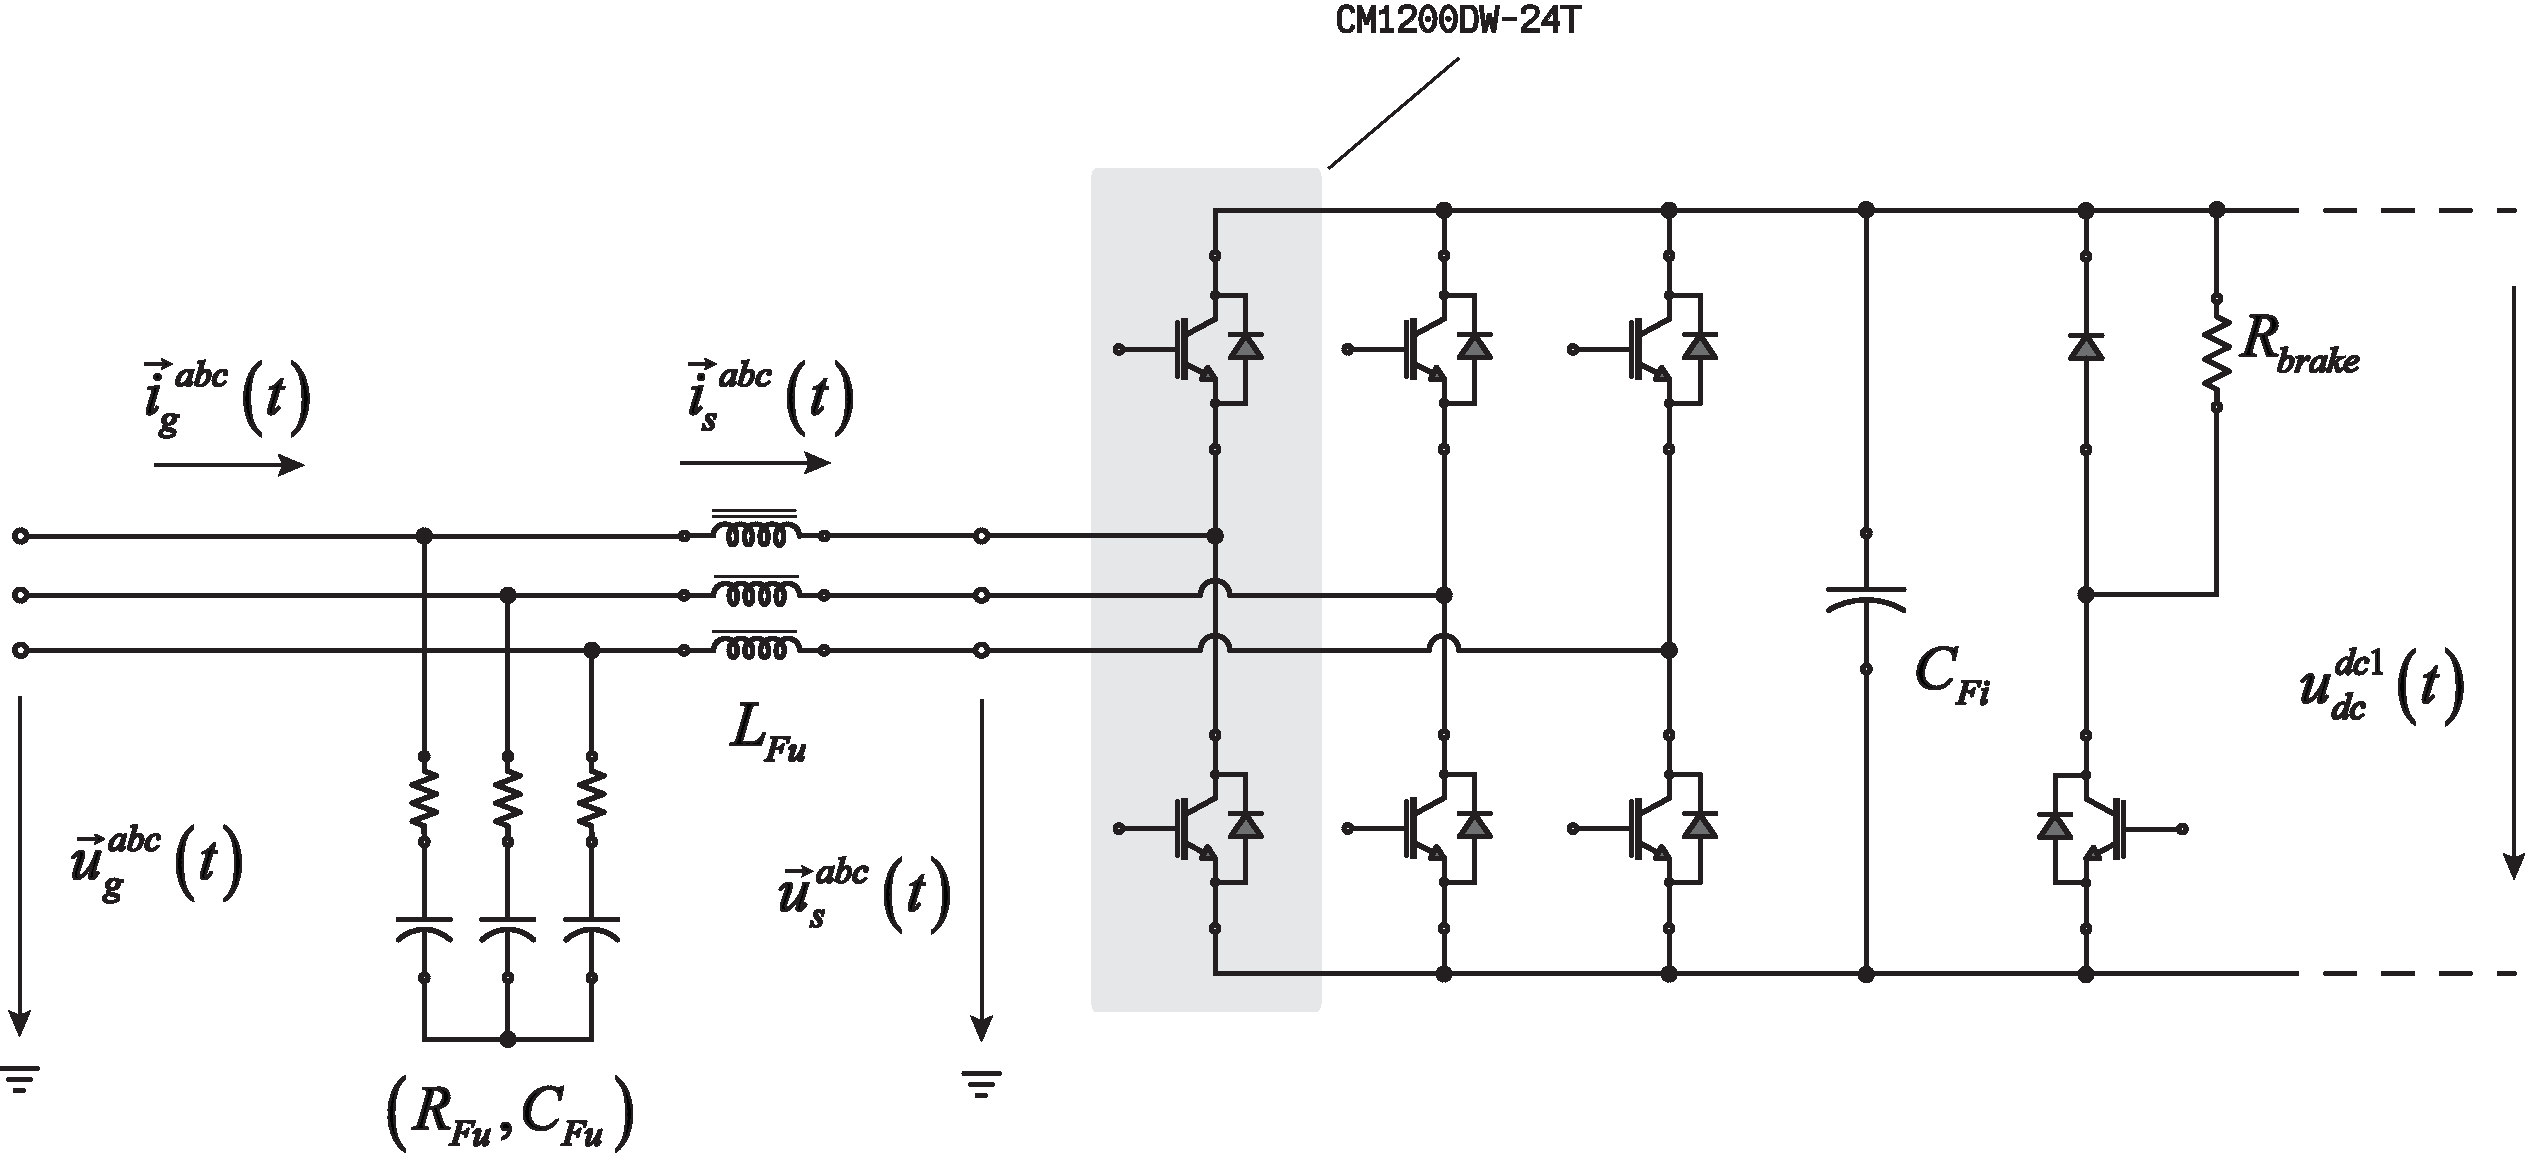
\includegraphics[width = 500pt, 
	keepaspectratio]{figures/arc/afe.pdf}
	\captionsetup{width=.75\textwidth}
	\caption{Active Front End stage with LC filter layout.}
	\label{fig:afe} 
\end{figure}

\begin{figure}[H]
	\centering
	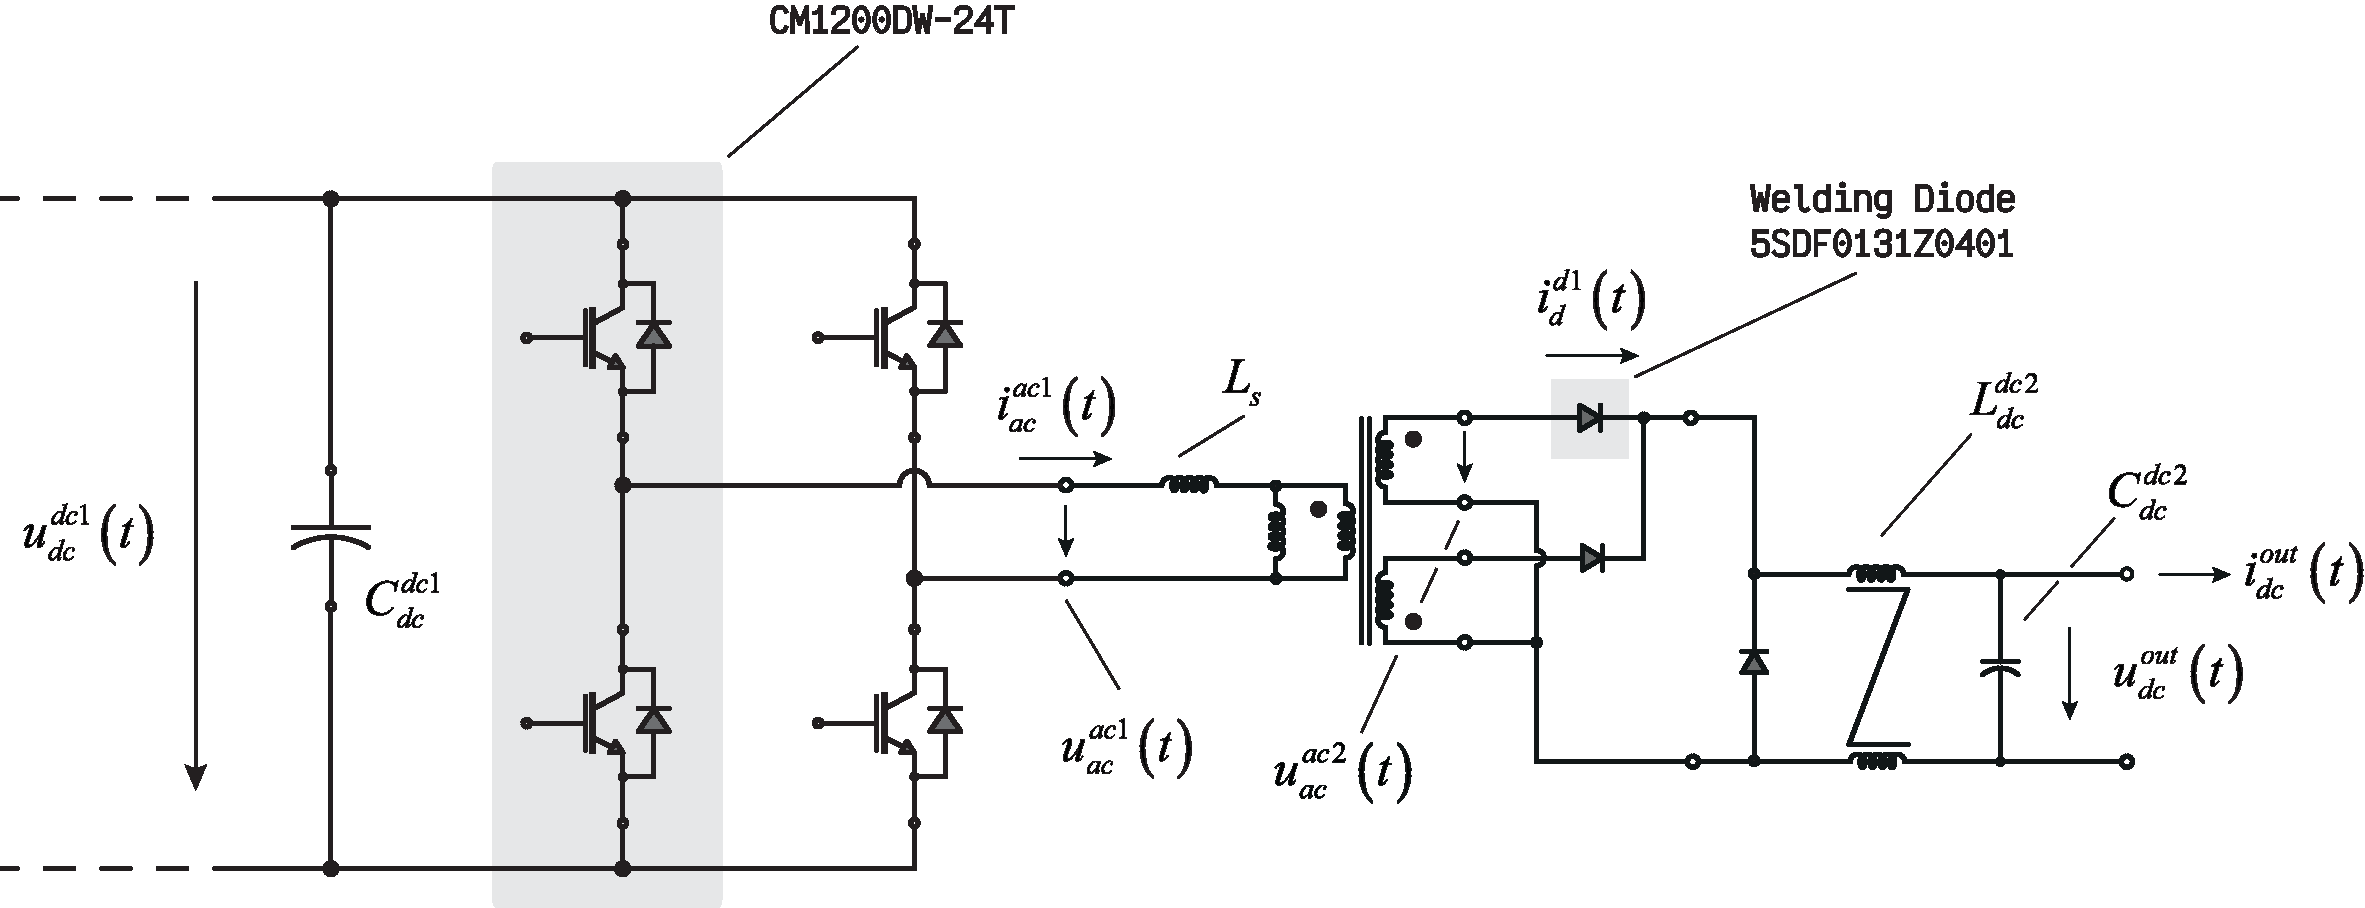
\includegraphics[width = 500pt, 
	keepaspectratio]{figures/arc/phase_shifted_full_bridge_converter_2.pdf}
	\captionsetup{width=.75\textwidth}
	\caption{Full Bridge Converter layout.}
	\label{fig:psfbc} 
\end{figure}

%\begin{figure}[H]
%	\centering
%	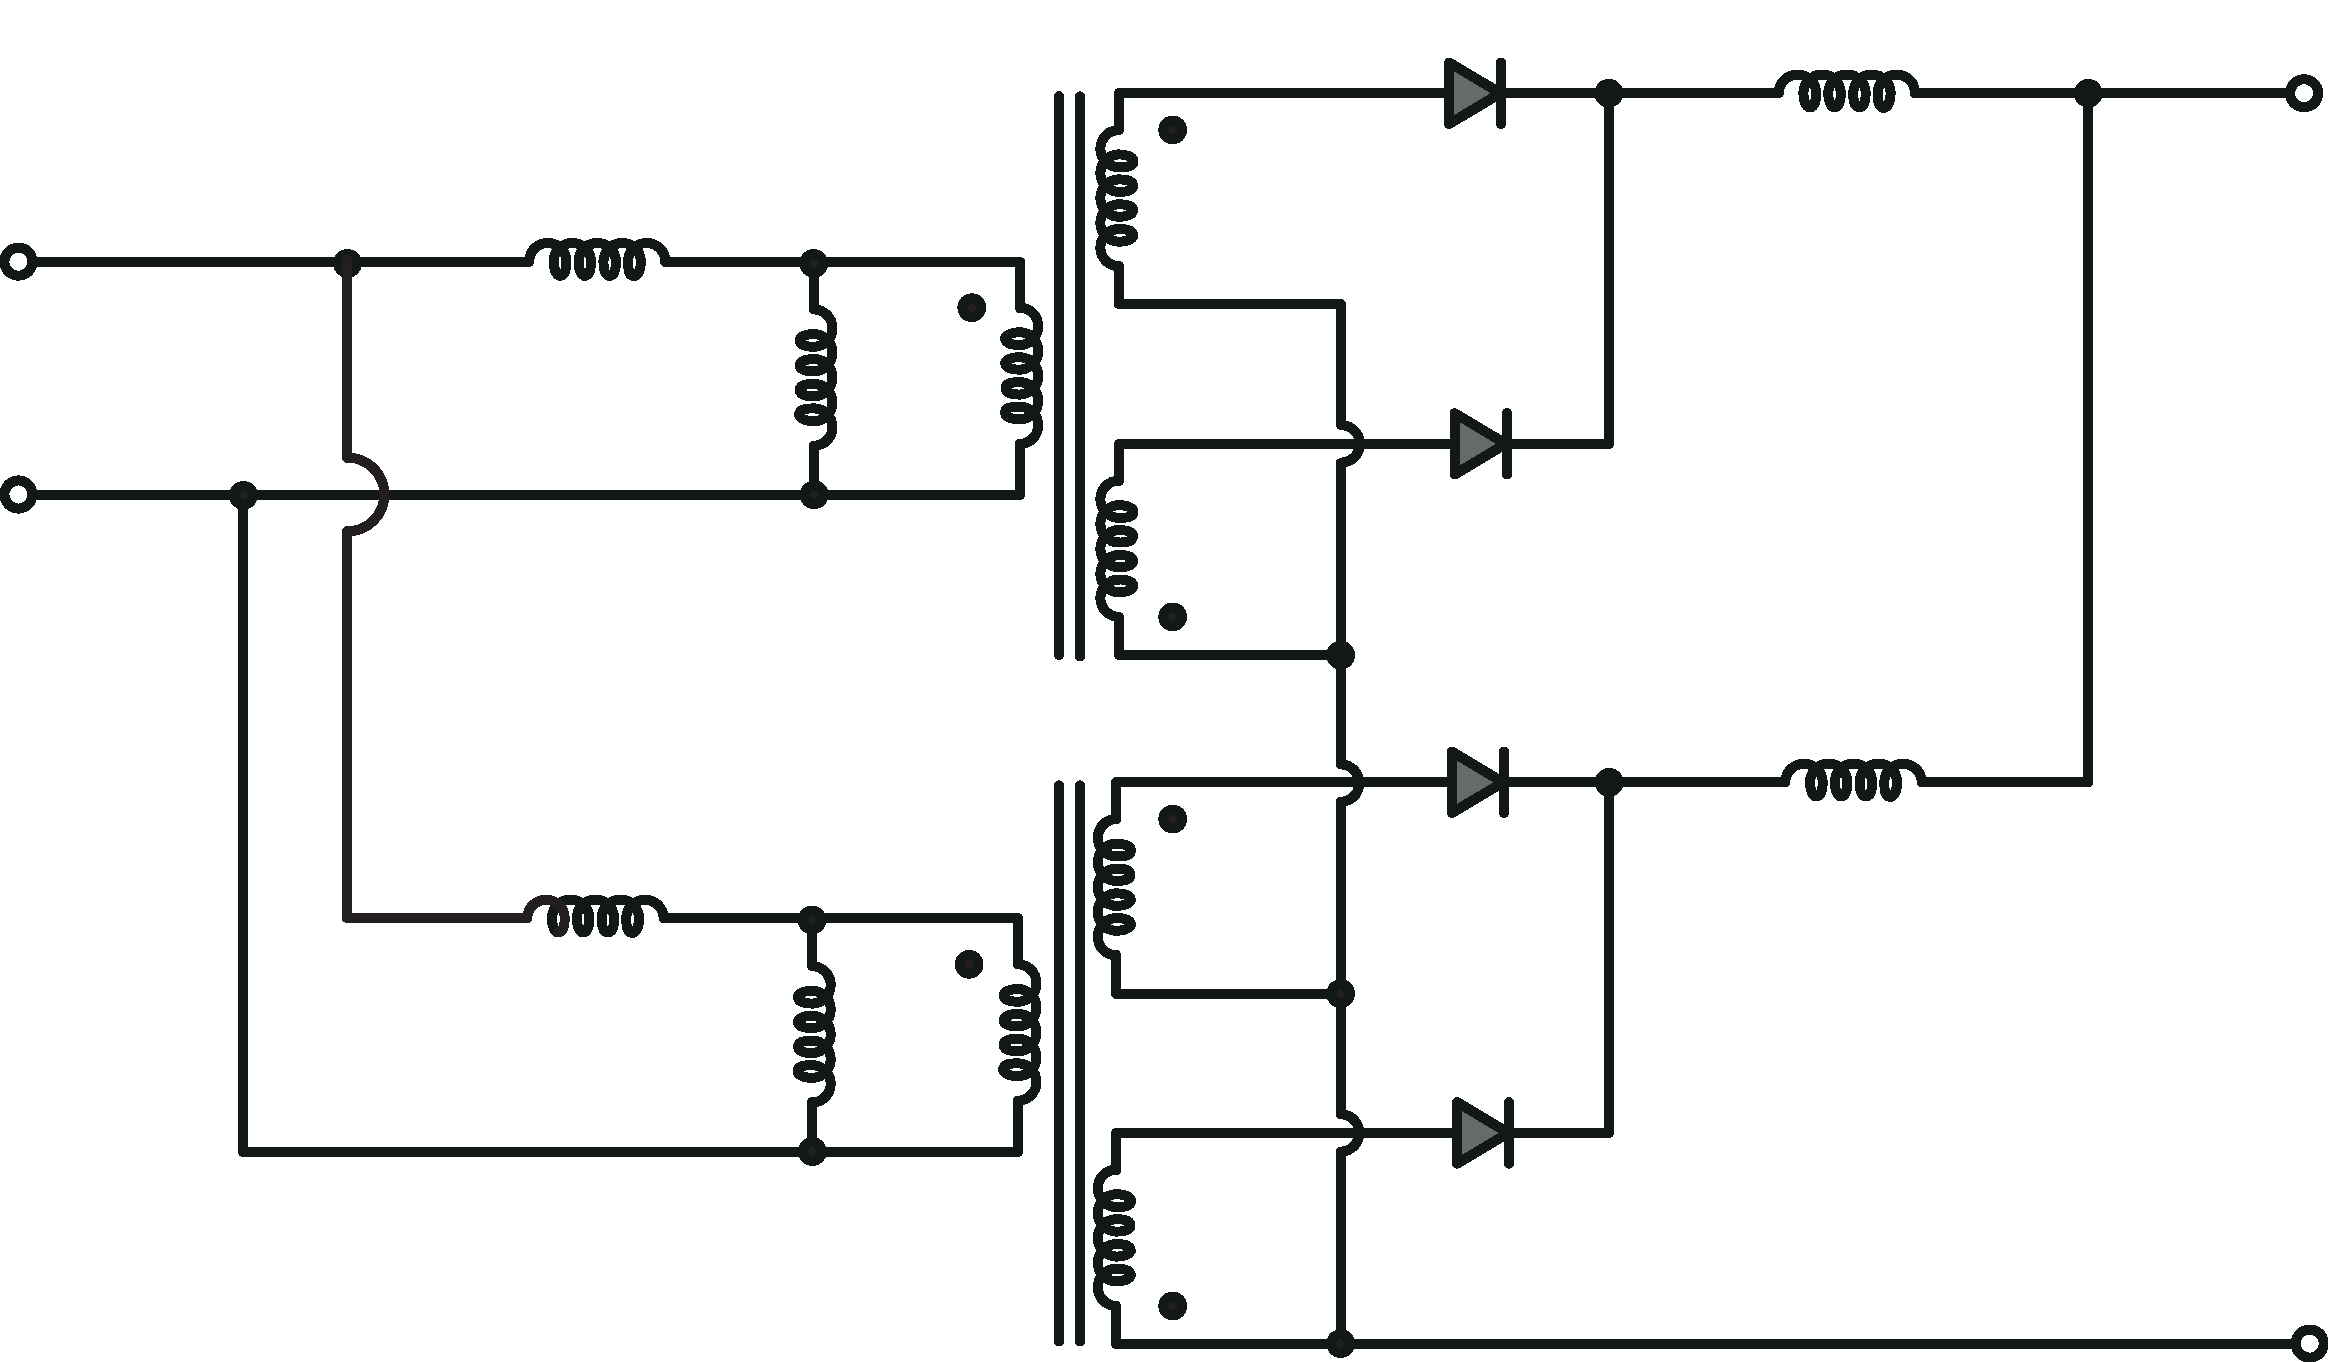
\includegraphics[width = 325pt, 
%	keepaspectratio]{figures/arc/HF-TR.pdf}
%	\captionsetup{width=.75\textwidth}
%	\caption{Details of the high frequency transformer with shared output inductance.}
%	\label{fig:hftr} 
%\end{figure}

The source inductance $L_\text{grid}$, determined by the grid short-circuit capacity
at the point of common coupling (\SI{15}{\kilo\ampere}), represents the
dominant upstream impedance seen by the AFE stage.
\begin{figure}[H]
	\centering
	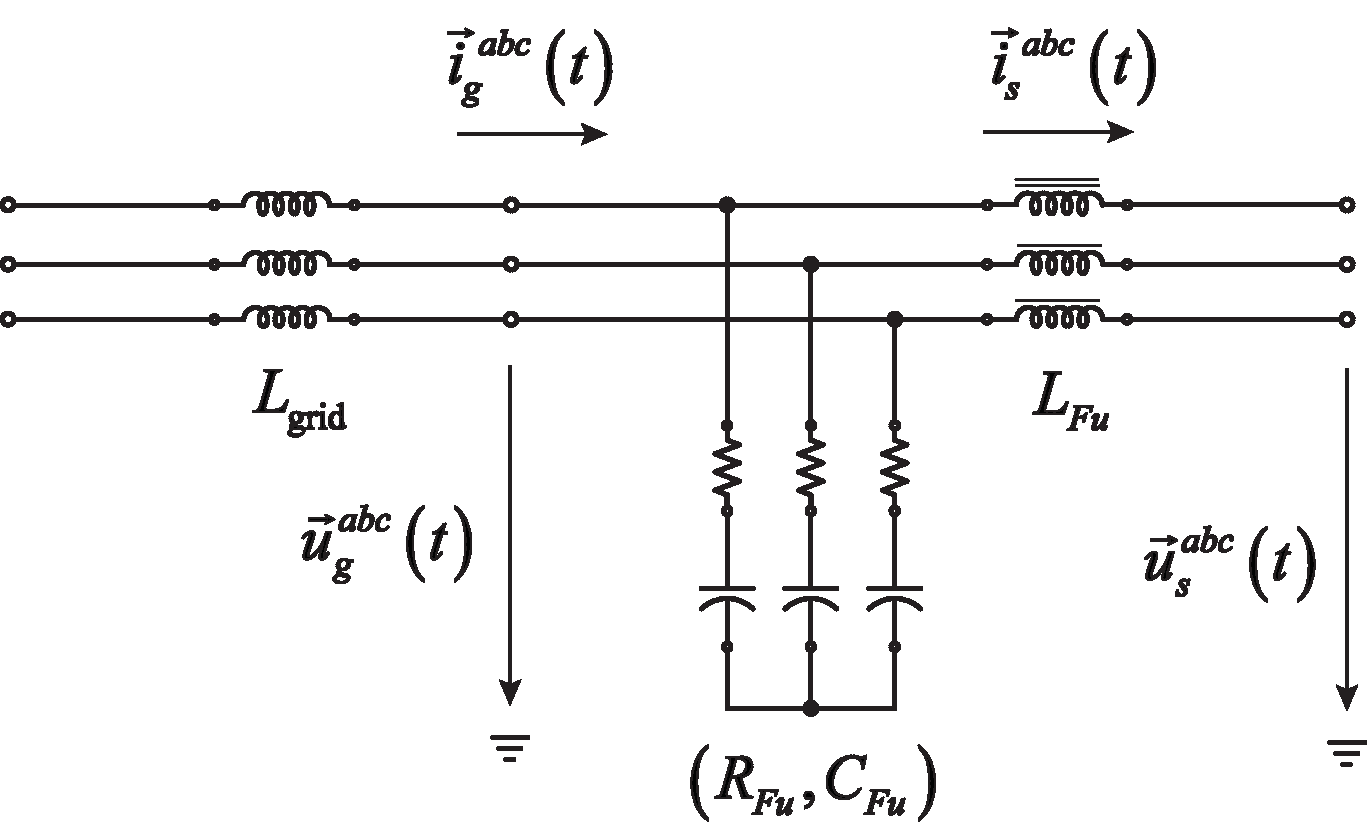
\includegraphics[width = 275pt, 
	keepaspectratio]{figures/arc/afe_grid_filter.pdf}
	\captionsetup{width=.75\textwidth}
	\caption{LCL filter built using the point of common coupling (PCC) inductance.}
	\label{fig:afe_grid_filter} 
\end{figure}
\begin{figure}[H]
	\centering
	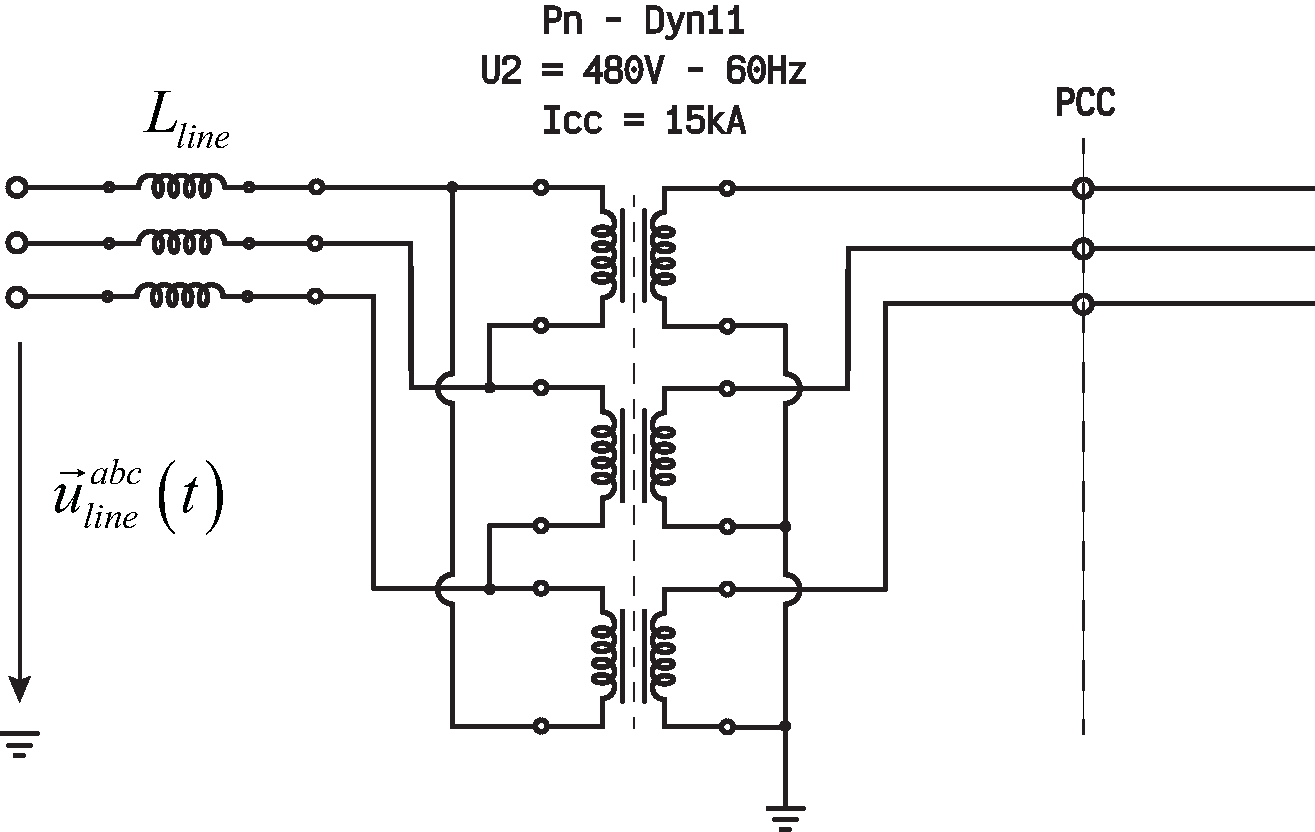
\includegraphics[width = 275pt, 
	keepaspectratio]{figures/arc/input_line.pdf}
	\captionsetup{width=.75\textwidth}
	\caption{Line representation.}
	\label{fig:line_representation} 
\end{figure}

\section{Power Supply Design}\label{sec:topology}

List of the power supply components and related sizing. 

 \begin{center}	
	\onehalfspacing
	\begin{longtable}{p{0.2\linewidth}|p{0.2\linewidth}|p{0.2\linewidth}|p{0.25\linewidth}}
		\captionsetup{width=0.65\textwidth, font=small}
		\caption{Component design.}
		\label{table:design} \\
		\toprule
		\textbf{component} & \textbf{Nominal data}  & \textbf{Design criteria data}  & \textbf{description} \\
		\midrule
		AFE $L_\text{Fu}$ & $L_\text{Fu} = \SI{330}{\micro\henry}$ & $I_\text{nom} = \SI{450}{\ampere}$ rms & liquid cooled \\	
		\midrule	
		AFE $C_\text{Fu}$ & $C_\text{Fu} = \SI{200}{\micro\farad}-\SI{360}{\micro\farad}$ & $U_\text{nom} = \SI{285}{\volt}$ rms, $I_\text{nom} = \SI{44}{\ampere}$ rms & film capacitor \\		
		\midrule
		AFE $R_\text{CFu}$ & $R_\text{CFu} = \SI{50}{\milli\ohm}$ & $P_\text{nom} = \SI{50}{\watt}$ & low inductance resistors \\
		\midrule
		AFE $L_\text{grid}$ & $L_\text{grid} = \SI{50}{\micro\henry}$ &  & from grid \\
		\midrule
		AFE IGBT module power losses & CM1200DW-24T, $R_g = \SI{1.15}{\ohm}$, $f_\text{pwm} = \SI{4}{\kilo\hertz}$ & $P_\text{loss} = \SI{1200}{\watt}$ per module under worst condition  & liquid cooled \\
		\midrule
		AFE DClink Capacitor & $C_\text{Fi} = \SI{2.4}{\milli\farad}$ & $U_\text{nom} = \SI{900}{\volt}$  & film capacitor \\
		\midrule
		FBC Input Capacitor & $C_\text{dc}^\text{dc1} = \SI{1.2}{\milli\farad}$ & $U_\text{nom} = \SI{900}{\volt}$  & film capacitor \\
		\midrule
		FBC IGBT module power losses & CM1200DW-24T, $t_{dt} = \SI{3}{\micro\second}$, $f_\text{pwm} = \SI{10}{\kilo\hertz}$ & $P_\text{loss} = \SI{1200}{\watt}$ per module under worst condition & liquid cooled \\
		\midrule
		HF Trafo series inductance & $L_s = \SI{8}{\micro\henry}$ & center tapped transformer, $f_\text{pwm} = \SI{10}{\kilo\hertz}$ & \\
		\midrule
		HF Trafo Primary Current & $I_1 = \SI{690}{\ampere}$ &  & RMS value for sizing  \\		
		\midrule
		HF Trafo Primary Voltage & $U_1 = \SI{680}{\volt}$ &  &  RMS value for sizing \\		
		\midrule
		HF Trafo Secondary Current & $I_2 = \SI{8400}{\ampere}$ per system &  & RMS value for sizing \\
		\midrule
		HF Trafo Secondary Voltage & $U_2 = \SI{35}{\volt}$ per system &  & RMS value for sizing \\
		\midrule
		Diode Rectifier Power losses & 5SDF-0131Z0401 &   $P_\text{loss} =  \SI{6}{\kilo\watt}$, $I_d^m = \SI{3000}{\ampere}$ per diode & Clamped plate and Snubbers \\
		\midrule
		FBC $L_\text{dc}^\text{dc2}$ & $L_\text{dc}^\text{dc2} = \SI{0.4}{\micro\henry}$ & $I_\text{nom} = \SI{12}{\kilo\ampere}$ & in air, maybe from bus bar partial loop inductance \\
		\midrule
		FBC $C_\text{dc}^\text{dc2}$ & $C_\text{dc}^\text{dc2} = \SI{50}{\milli\farad}$ & $I_\text{nom} = \SI{350}{\ampere}$ rms & film (mandatory) \\
		\bottomrule
	\end{longtable}
\end{center}

\subsection{General design aspects}
Here a list of preliminary assumptions, and design choices:
\begin{itemize}
	\item[--] Nominal AFE power rate has been selected at $P_\text{nom}^\text{afe} = \SI{325}{\kilo\watt}$.
	\item[--] Nominal AFE stack current has been selected at $I_\text{nom}^\text{afe} = \SI{435}{\ampere}$ (rms).
	\item[--] AFE pwm switching frequency has been selected at $f_\text{pwm}^\text{afe} = \SI{4}{\kilo\hertz}$.
	\item[--] PS-FBC pwm switching frequency has been selected at $f_\text{pwm}^\text{fbc} = \SI{10}{\kilo\hertz}$ (operative frequency of the transformers).
	\item[--] The overall architecture, AFE+PS-FBC has been simulated assuming \textbf{CM1200DW-24T} ($T_j^\text{max} = \SI{175}{\celsius}$) as switching device. Maximum power loss for each \textbf{module} remains below than \SI{1.4}{\kilo\watt} along the worst operative condition. 
\end{itemize}

\noindent\textbf{Remark} - the secondary rectifier stage of the PS-FBC has been implemented using
slow-recovery diodes; the Simscape model has been updated accordingly to
include a full diode model.

The selected switching frequency of \SI{10}{\kilo\hertz} represents a design compromise between volume and sound emission. The choice of \SI{10}{\kilo\hertz} allows the use of ferrite core.

%A ferrite-core transformer at this frequency results
%in an excessively large and heavy magnetic component, whereas an
%amorphous-iron core, while better suited to lower frequencies, introduces
%significant acoustic noise at and around the switching frequency.
%
%An improved solution — not evaluated in the present work — would consist
%of replacing the slow-recovery diodes with fast-recovery rectifiers,
%adopting SiC MOSFETs on the primary side, and increasing the switching
%frequency to \SI{10}{\kilo\hertz}. This would allow the use of a
%compact ferrite-core transformer while maintaining acceptable switching
%losses.

\subsection{AFE-LCL filter topology}
As shown in Figure~\ref{fig:afe_grid_filter} the active-front-end is interfaced to the grid via an LCL filter (even if the input inductor ($L_\text{Fu}$) is mandatory for the conversion). In this context and assuming an $I_\text{cc}=\SI{15}{\kilo\ampere}$ which results into a $L_\text{grid} \approx\SI{54}{\micro\henry}$.

\noindent\textbf{Remark} - the LCL filter will be composed by an LRC filter ($L_\text{Fu}$, $C_\text{Fu}$, and $R_\text{CFu}$) plus the point of common coupling inductance ($L_\text{grid}$).
The $R_\text{CFu} = \SI{50}{\milli\ohm}$ is basically used as damping and in general helps to achieve harmonics compliance in the scenario of power generation where, as according to IEEE519, the harmonic limits are reduced by a factor of two.

\subsection{AFE DClink}
The DClink capacitor has been selected as follows
\begin{itemize}
	\item[--] Film capacitor DClink bank;
	\item[--] DClink bank value $C_{Fi} \approx \SI{2.4}{\milli\farad}–\SI{3.6}{\milli\farad}$;	
	\item[--] DClink bank rated voltage $U_{C_\text{Fi}}^\text{nom} \approx \SI{900}{\volt}–\SI{1300}{\volt}$.
\end{itemize}

\subsection{Phase Shift Full bridge Converter topology}

\noindent\textbf{Rectifier stage} - rectifier stage is implemented using the component 5SDF-0131Z0401. In order to evaluate the effect of the reverse recovery current, diode simscape model has been implemented using the junction charge model. \\

\noindent\textbf{HF Transformer stage} - The series inductance $L_s$, comprising the transformer leakage inductance
$L_{lk}$ and an optional external inductor $L_{ext}$, plays a central role in the operation of the Phase-Shift Full Bridge Converter (PS-FBC). It stores the energy required to charge and discharge the IGBT output capacitance $C_{oss}$ during the dead-time interval, thereby enabling Zero-Voltage Switching (ZVS). Furthermore, $L_s$ governs the power transferred between primary and secondary according to the phase-shift angle $\varphi(t)$, and provides inherent $\mathrm{d}i/\mathrm{d}t$ limiting during fault conditions.

Transformer has been sized as follows
\begin{itemize}
	\item[--] centre-tapped transformer with a turns ratio of $n_1/n_2 = n_1/n_3 = 17$;
	\item[--] $L_s = \SI{8}{\micro\henry}$ per transformer which represents a trade-off between ZVS range and maximum power delivery;
\end{itemize}

\subsection{AFE and FBC Devices}
The primary full-bridge stage as well as the three phase inverter are built using the LV100 module CM12000DW-24T which has a maximum junction temperature $T_j^\text{max} = \SI{175}{\celsius}$.

\subsection{Overall Efficiency}

\noindent\textbf{AFE} --- An AFE with a rated current of \SI{450}{\ampere},
a switching frequency of \SI{4}{\kilo\hertz}, and a DC-link voltage of
\SI{750}{\volt} requires liquid cooling. The overall AFE losses are
estimated at approximately \SI{5}{\kilo\watt}, comprising \SI{1.4}{\kilo\watt}
in the commutation inductance $L_\text{Fu}$ and \SI{3.6}{\kilo\watt} in the
IGBT modules.

\noindent\textbf{FBC} --- Similar considerations apply to the FBC stage.
The full-bridge switching losses are estimated at approximately
\SI{3}{\kilo\watt} under the worst-case operating condition.

\noindent\textbf{HF-TR} --- For the HF transformer, a total loss of
\SI{5}{\kilo\watt} is assumed, accounting for both core and winding losses.

\noindent\textbf{Rectifier} --- With two diode modules each carrying
\SI{6}{\kilo\ampere}, the total rectifier conduction loss amounts to
approximately \SI{12}{\kilo\watt}.

\noindent\textbf{Bus Bars} --- overall bus bar connection power losses has been assumed approximately \SI{2}{\kilo\watt}.

\noindent The individual loss contributions are summarised below:
\begin{itemize}
	\item[--] $P_\text{loss}^\text{AFE}   = \SI{3.6}{\kilo\watt}$;
	\item[--] $P_\text{loss}^\text{LFu}   = \SI{1.4}{\kilo\watt}$;
	\item[--] $P_\text{loss}^\text{FBC}   = \SI{3.0}{\kilo\watt}$;
	\item[--] $P_\text{loss}^\text{HF-TR} = \SI{5.0}{\kilo\watt}$;
	\item[--] $P_\text{loss}^\text{RECT}  = \SI{12.0}{\kilo\watt}$;	
	\item[--] $P_\text{loss}^\text{BusBars}  = \SI{2.0}{\kilo\watt}$;
\end{itemize}

\noindent\textbf{Remark} --- The total estimated loss is
$P_\text{loss}^\text{tot} \approx \SI{27}{\kilo\watt}$, corresponding to
an overall system efficiency of
$\eta = P_\text{out}/(P_\text{out}+P_\text{loss}^\text{tot})
= 300/(300+27) \approx \SI{91.7}{\percent}$,
which satisfies the requirement $\eta > \SI{90}{\percent}$.

\section{Simulation Results}\label{sec:sim}
Simulations have been performed at two working condition
\begin{itemize}
	\item[--] NLC: $u_\text{dc}^\text{out} = \SI{25}{\volt}$ and $i_\text{dc}^\text{out} = \SI{12}{\kilo\ampere}$;
	\item[--] NLH: $u_\text{dc}^\text{out} = \SI{10}{\volt}$ and $i_\text{dc}^\text{out} = \SI{12}{\kilo\ampere}$;
\end{itemize}

\subsection{Case scenario NLC}
This subsection presents the simulation results for the NLC case. The simulations report the voltages and currents of the main passive and active components, as well as the corresponding losses.

\begin{figure}[H]
	\centering
	\begin{subfigure}{0.5\textwidth}
		\centering
		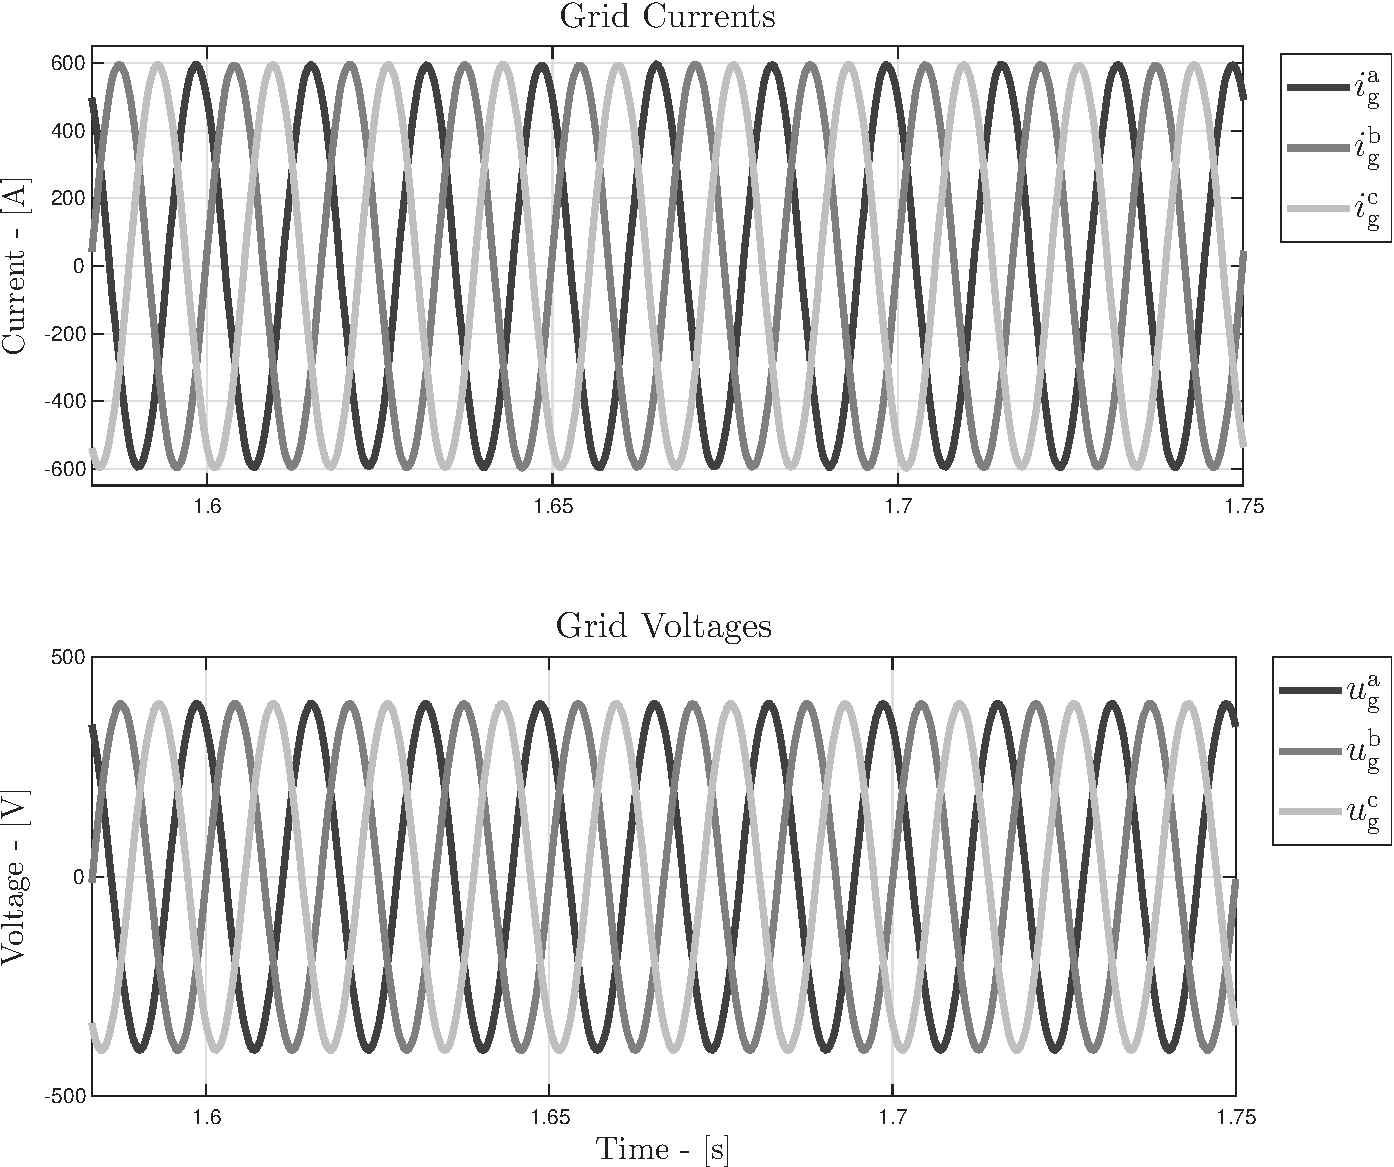
\includegraphics[width =225pt, angle = 0, 
		keepaspectratio]{figures/sim_results_7/grid_quantities.pdf}
		\captionsetup{width=0.95\textwidth, font=footnotesize}	
		\caption{Grid current waveform (top), and grid voltage waveform (bottom).}
		\label{}
	\end{subfigure}%
	\begin{subfigure}{0.5\textwidth}
		\centering
		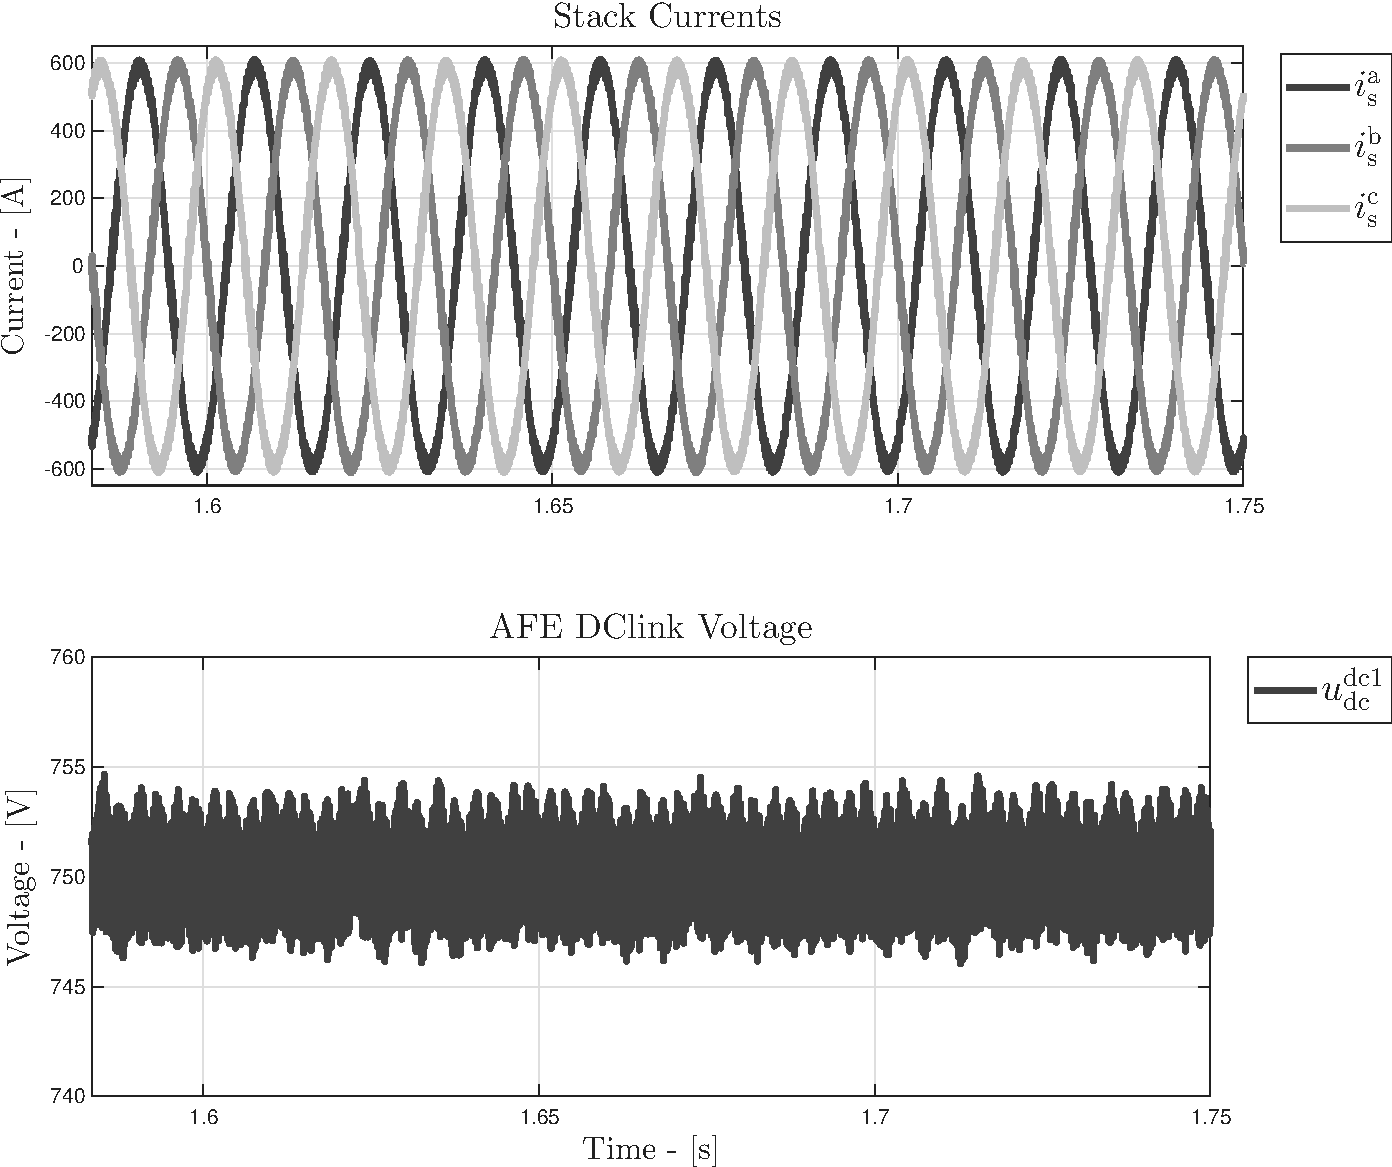
\includegraphics[width =225pt, angle = 0, 
		keepaspectratio]{figures/sim_results_7/afe_stack_quantities.pdf}
		\captionsetup{width=0.75\textwidth, font=footnotesize}	
		\caption{AFE-Stack current waveform (top), and AFE-DClink Voltage waveform (bottom).}
		\label{}
	\end{subfigure}
	\captionsetup{width=0.65\textwidth, font=small}	
	\caption{Grid and AFE stack quantities - case scenario NLC.}
	\label{}
\end{figure}

\begin{figure}[H]
	\centering
	\begin{subfigure}{0.5\textwidth}
		\centering
		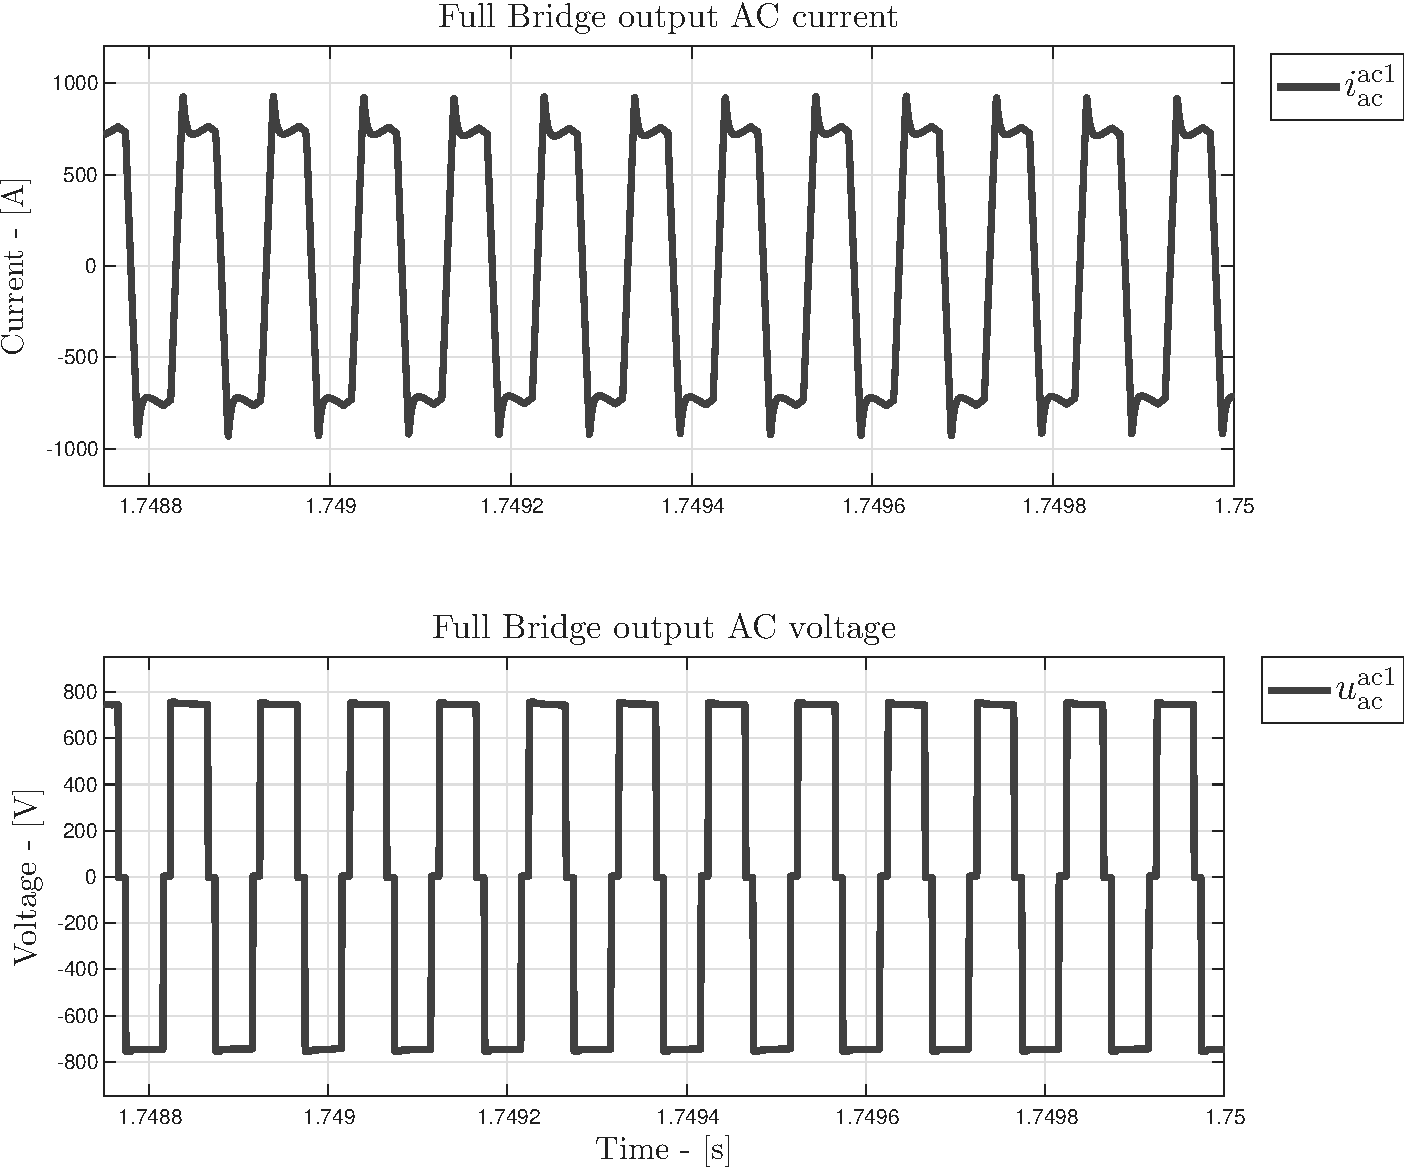
\includegraphics[width = 225pt, angle = 0, 
		keepaspectratio]{figures/sim_results_7/fbc_quantities_1.pdf}
		\captionsetup{width=0.95\textwidth, font=footnotesize}	
		\caption{Full Bridge output current (top), and output voltage (bottom).}
		\label{}
	\end{subfigure}%
	\begin{subfigure}{0.5\textwidth}
		\centering
		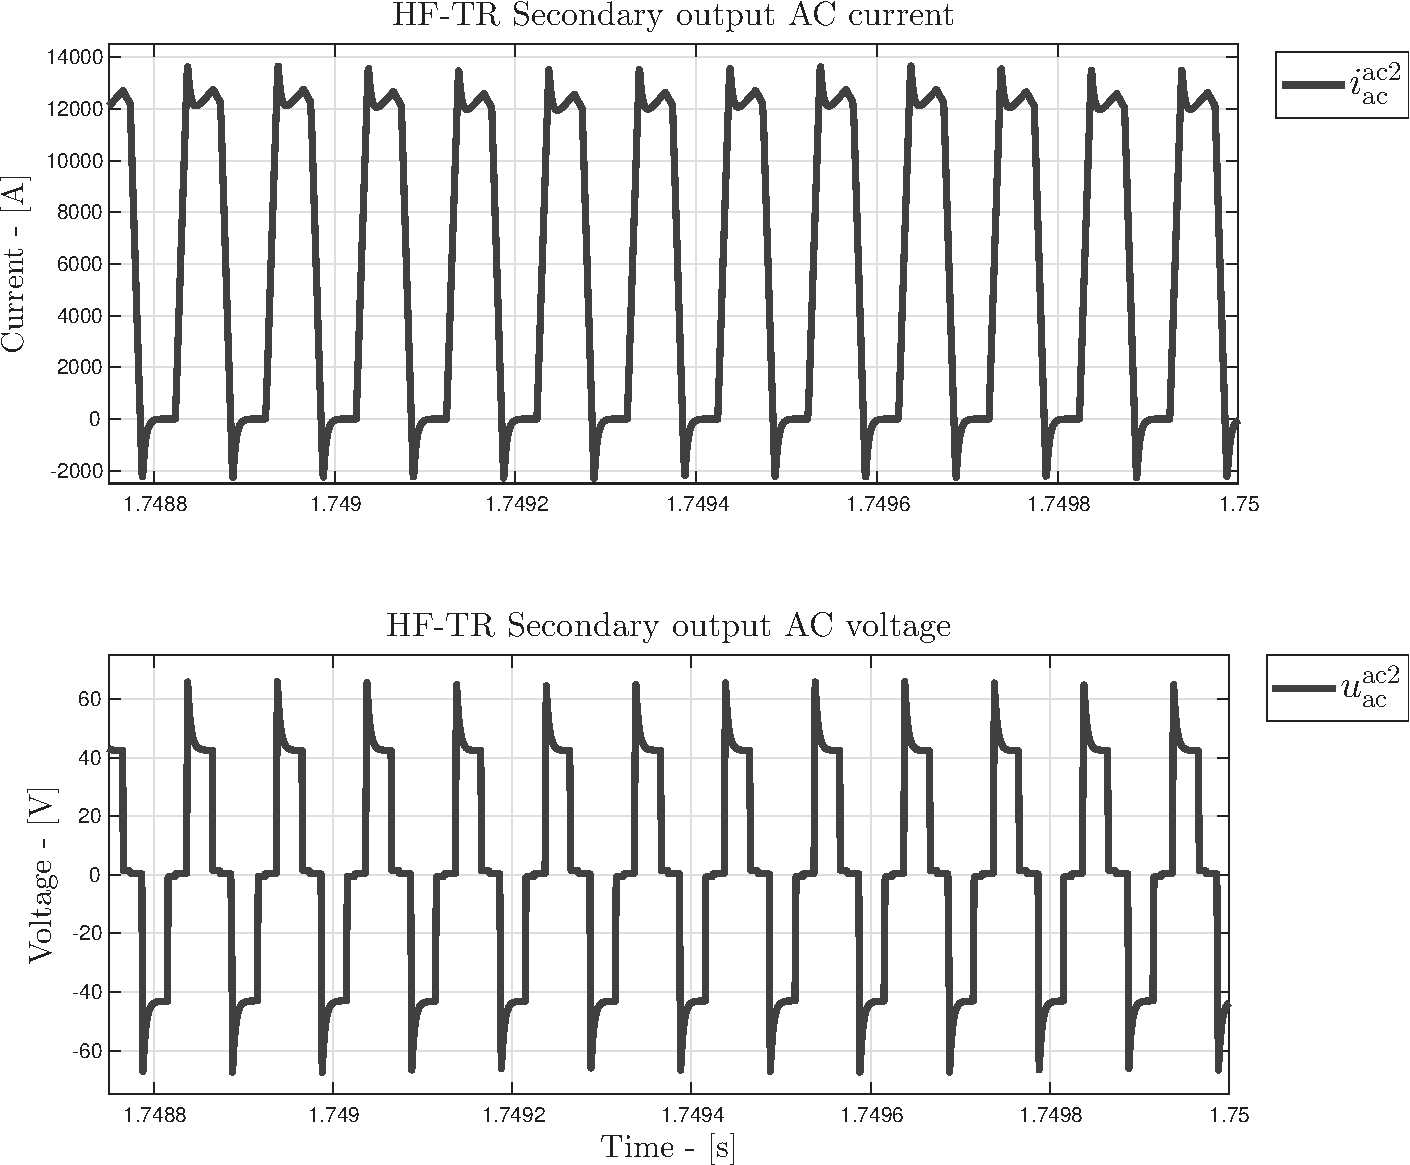
\includegraphics[width = 225pt, angle = 0, 
		keepaspectratio]{figures/sim_results_7/fbc_quantities_2.pdf}
		\captionsetup{width=0.75\textwidth, font=footnotesize}	
		\caption{HF-TR secondary current (top), and voltage (bottom).}
		\label{}
	\end{subfigure}
	\captionsetup{width=0.65\textwidth, font=small}	
	\caption{Full Bridge Converter quantities - case scenario NLC.}
	\label{}
\end{figure}

\begin{figure}[H]
	\centering
	\begin{subfigure}{0.5\textwidth}
		\centering
		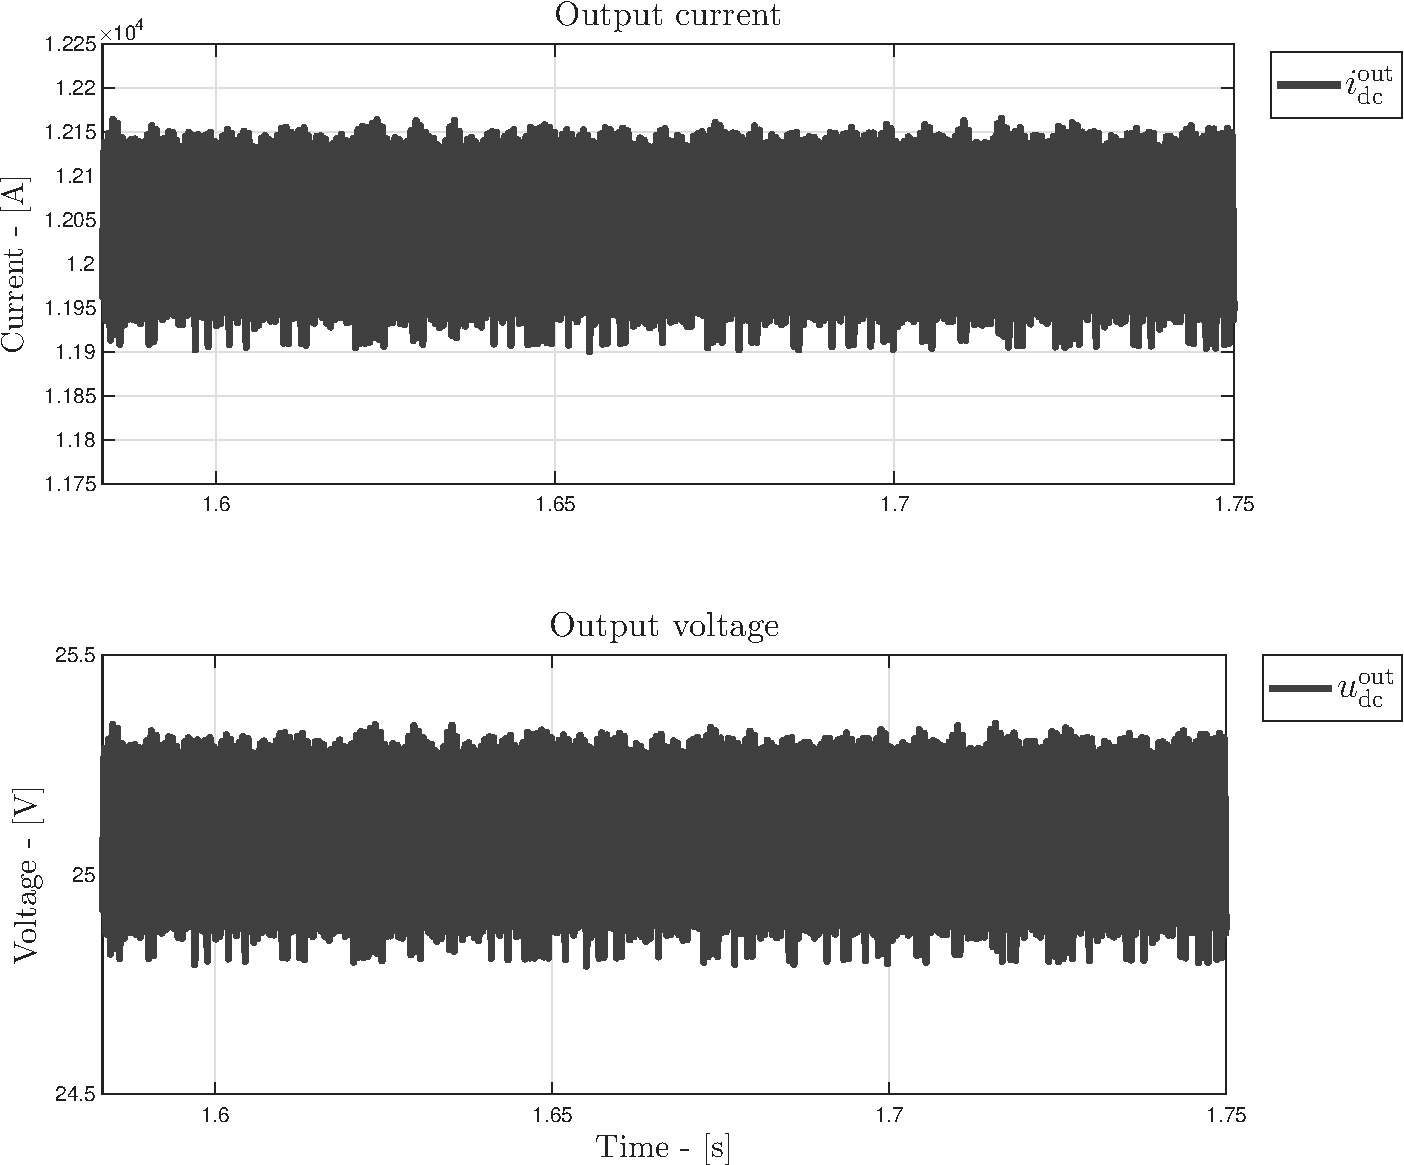
\includegraphics[width = 225pt, angle = 0, 
		keepaspectratio]{figures/sim_results_7/output_quantities.pdf}
		\captionsetup{width=0.5\textwidth, font=footnotesize}	
		\caption{Output current (top), and output voltage (bottom).}
		\label{}
	\end{subfigure}%
	\begin{subfigure}{0.5\textwidth}
		\centering
		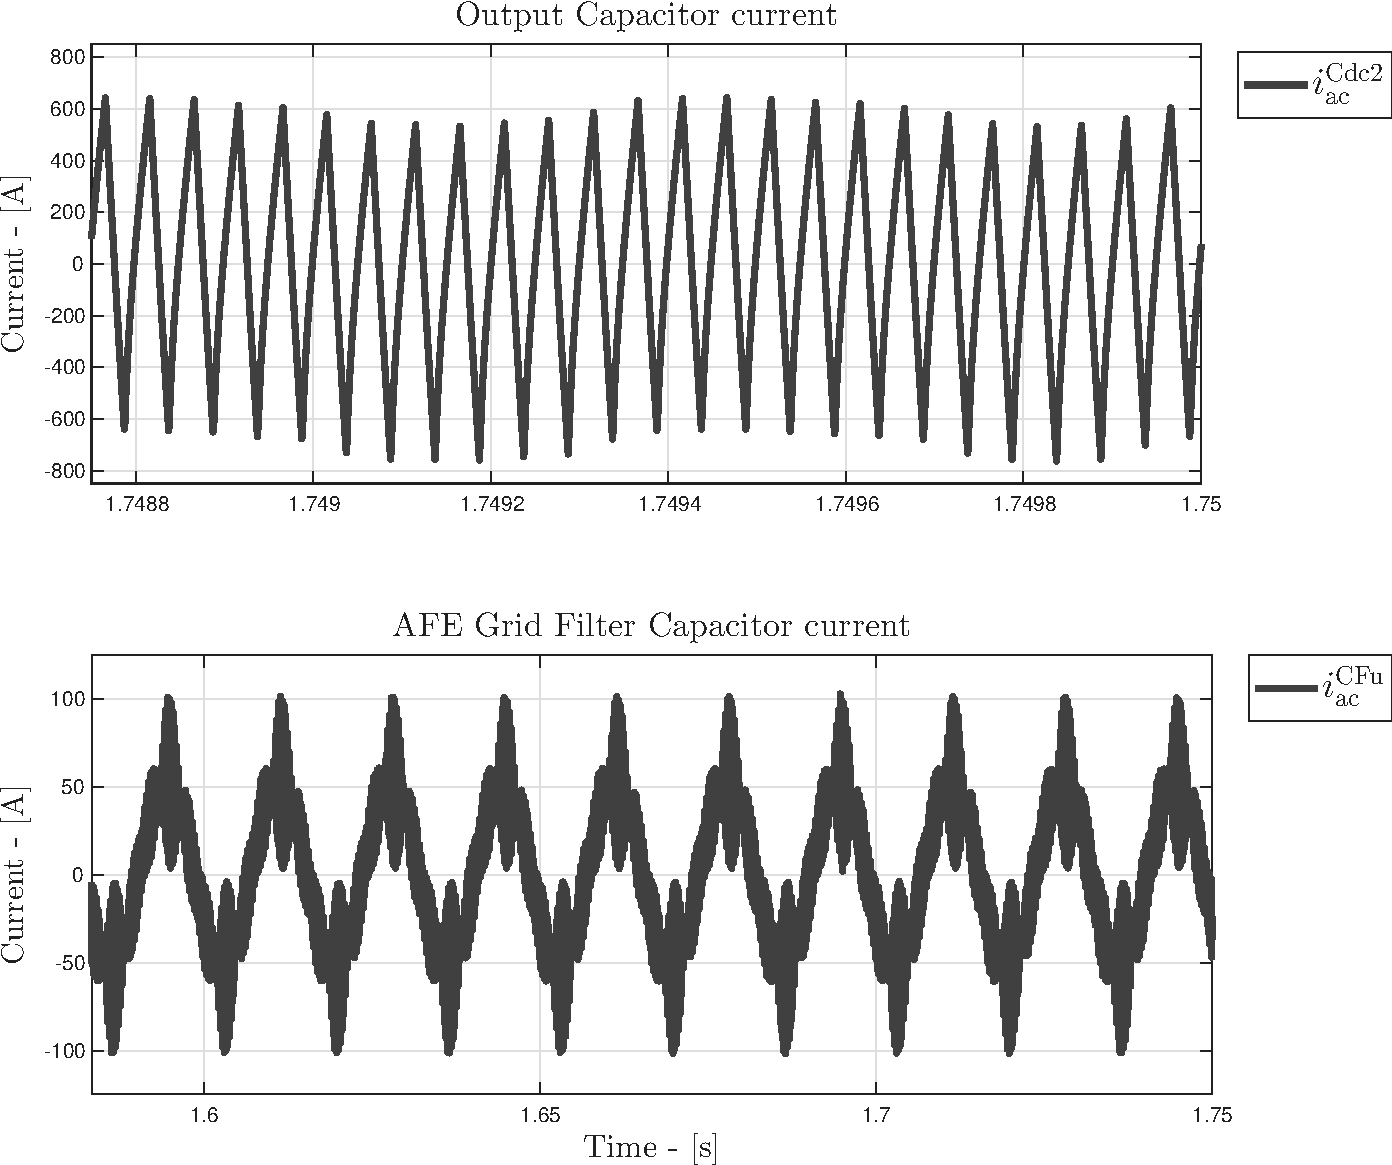
\includegraphics[width = 225pt, angle = 0, 
		keepaspectratio]{figures/sim_results_7/capacitors_currents.pdf}
		\captionsetup{width=0.95\textwidth, font=footnotesize}	
		\caption{Output filter capacitor current (top), and AFE grid filter capacitor current (bottom).}
		\label{}
	\end{subfigure}
	\captionsetup{width=0.65\textwidth, font=small}	
	\caption{Output quantities and capacitor filter currents - case scenario NLC.}
	\label{}
\end{figure}

\begin{figure}[H]
	\centering
	\begin{subfigure}{0.5\textwidth}
		\centering
		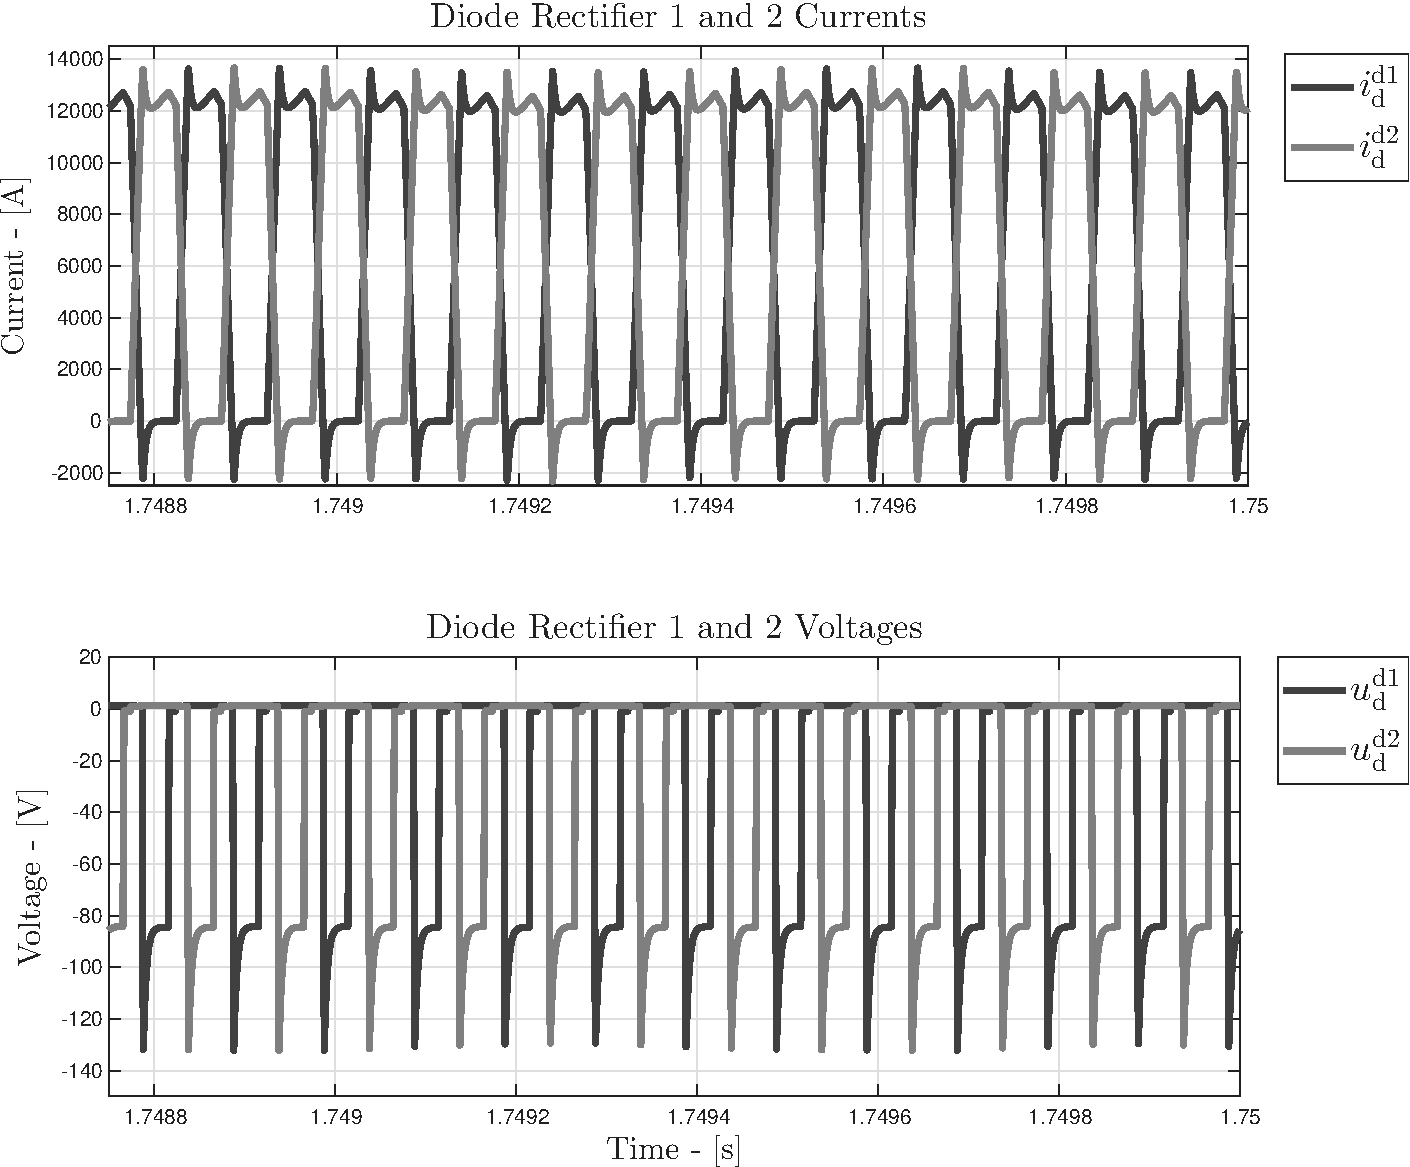
\includegraphics[width = 225pt, angle = 0, 
		keepaspectratio]{figures/sim_results_7/diode_rectifier.pdf}
		\captionsetup{width=0.75\textwidth, font=footnotesize}	
		\caption{Diode rectifiers current (top), and diode rectifiers voltage (bottom).}
		\label{}
	\end{subfigure}%
	\begin{subfigure}{0.5\textwidth}
		\centering
		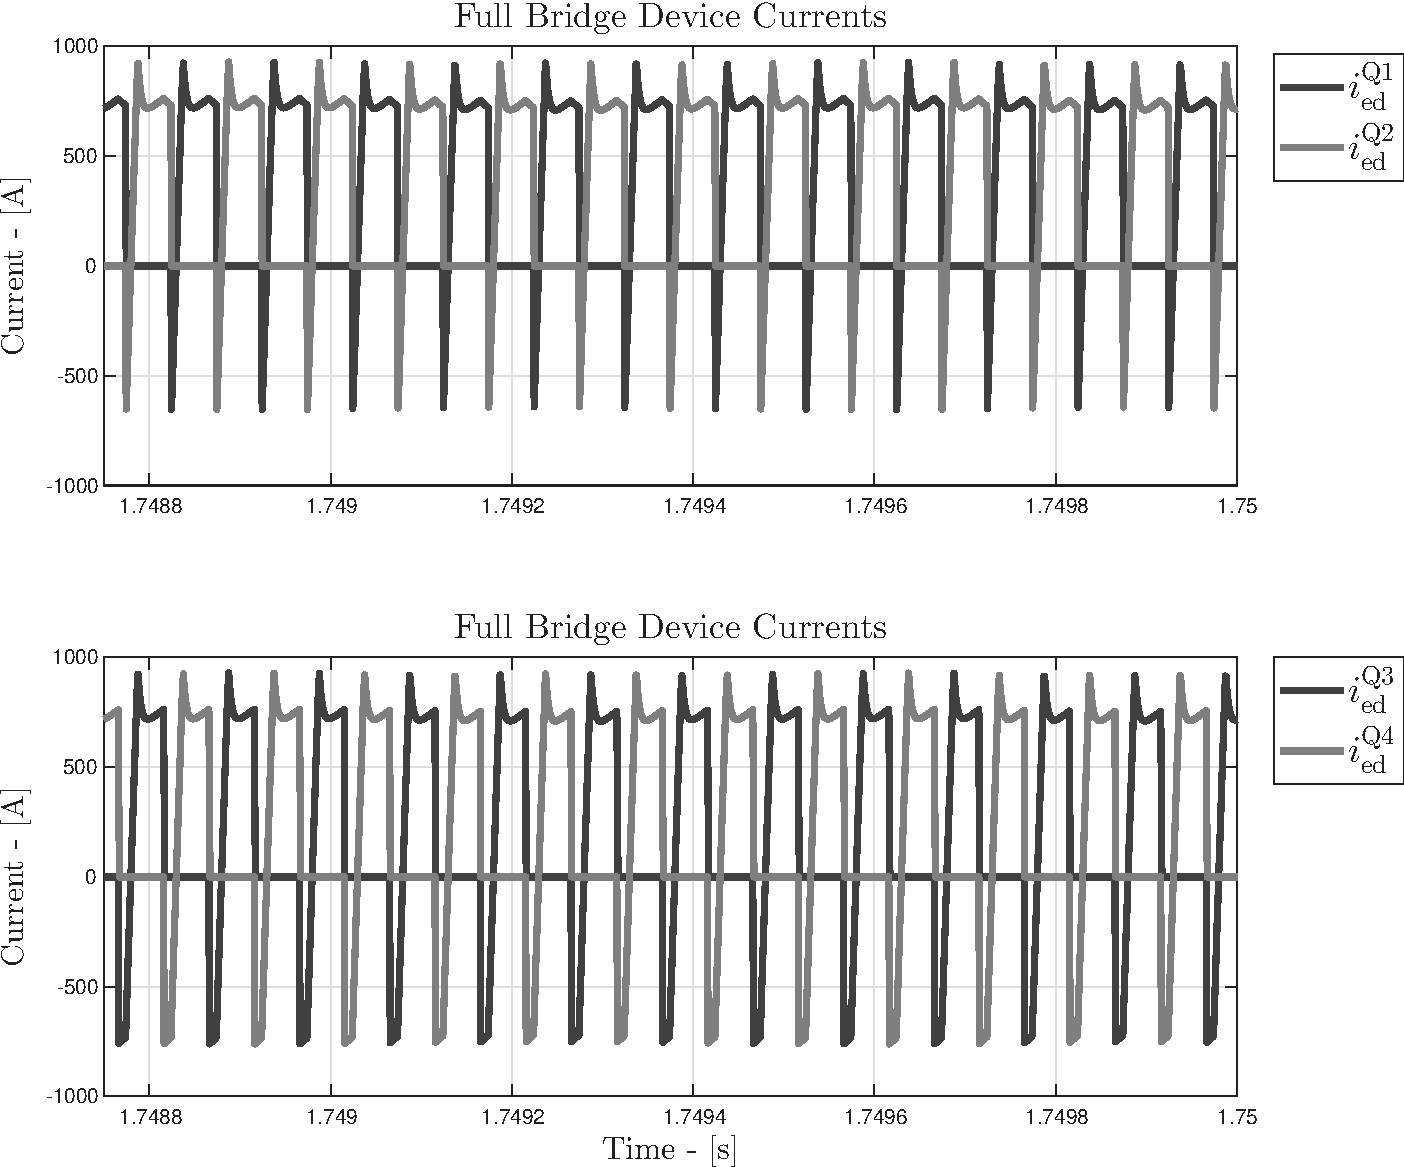
\includegraphics[width = 225pt, angle = 0, 
		keepaspectratio]{figures/sim_results_7/full_bridge_devices_quantities.pdf}
		\captionsetup{width=0.75\textwidth, font=footnotesize}	
		\caption{Full Bridge devices current first leg (top), and second leg (bottom).}
		\label{}
	\end{subfigure}
	\captionsetup{width=0.65\textwidth, font=small}	
	\caption{Full bridge devices current and diode rectifiers current - case scenario NLC.}
	\label{}
\end{figure}

\begin{figure}[H]
	\centering
	\begin{subfigure}{0.5\textwidth}
		\centering
		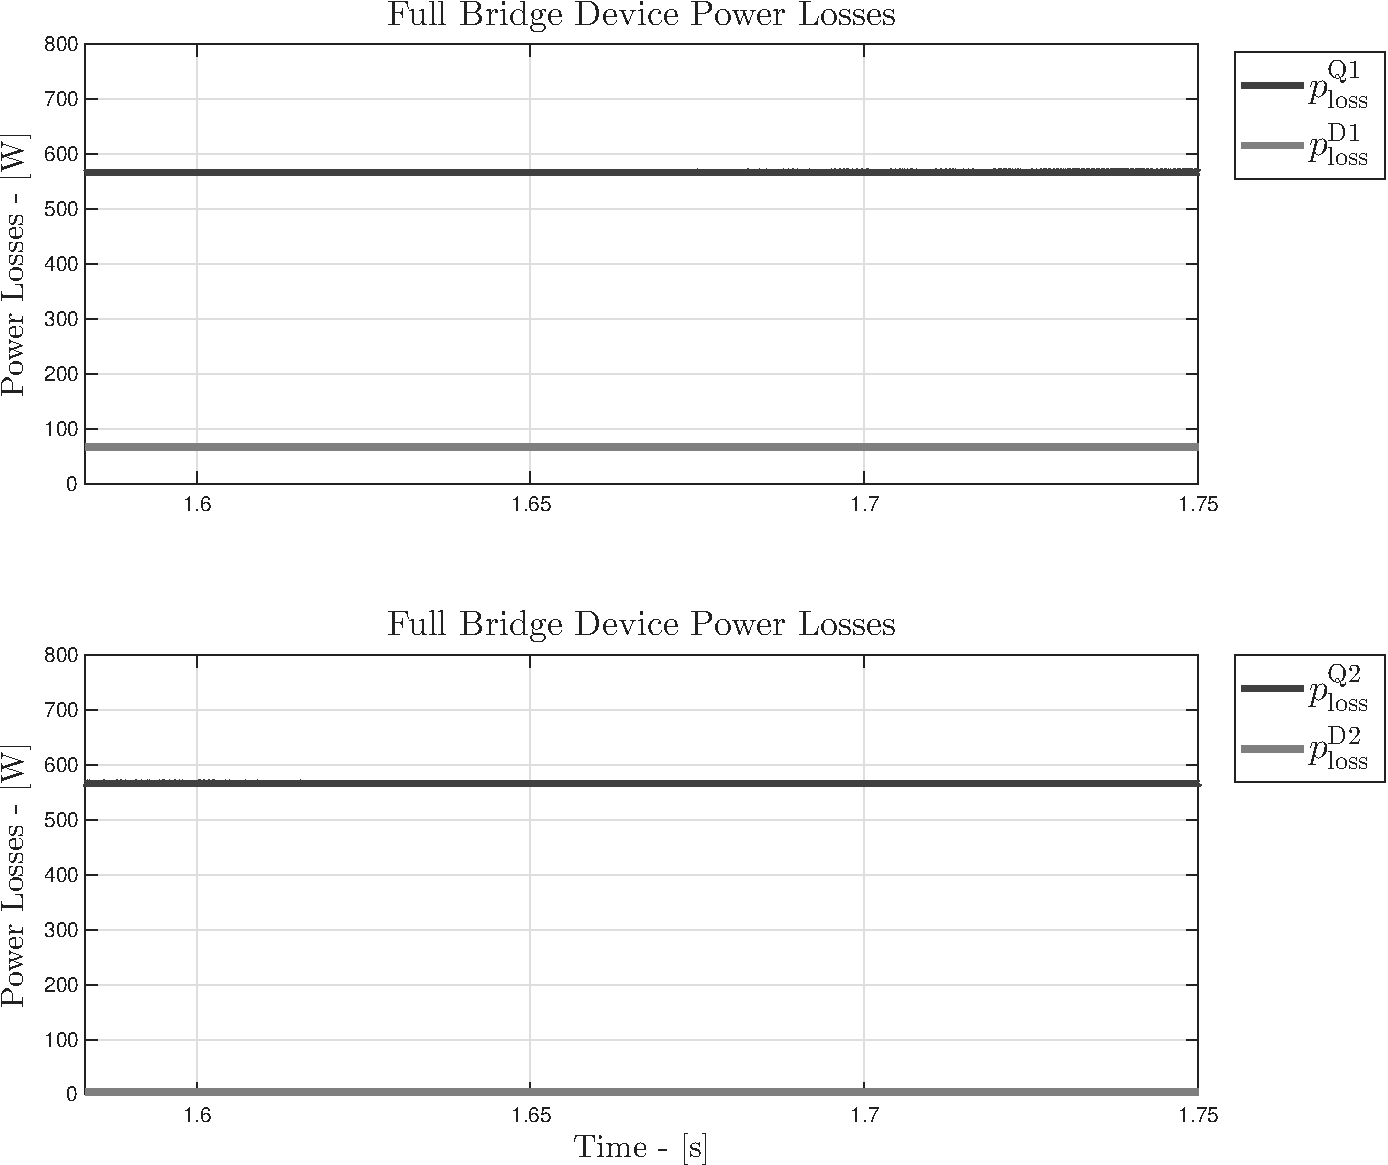
\includegraphics[width = 225pt, angle = 0, 
		keepaspectratio]{figures/sim_results_7/full_bridge_devices_power_losses_1.pdf}
		\captionsetup{width=0.75\textwidth, font=footnotesize}	
		\caption{Full Bridge device power losses (top), and (bottom).}
		\label{}
	\end{subfigure}%
	\begin{subfigure}{0.5\textwidth}
		\centering
		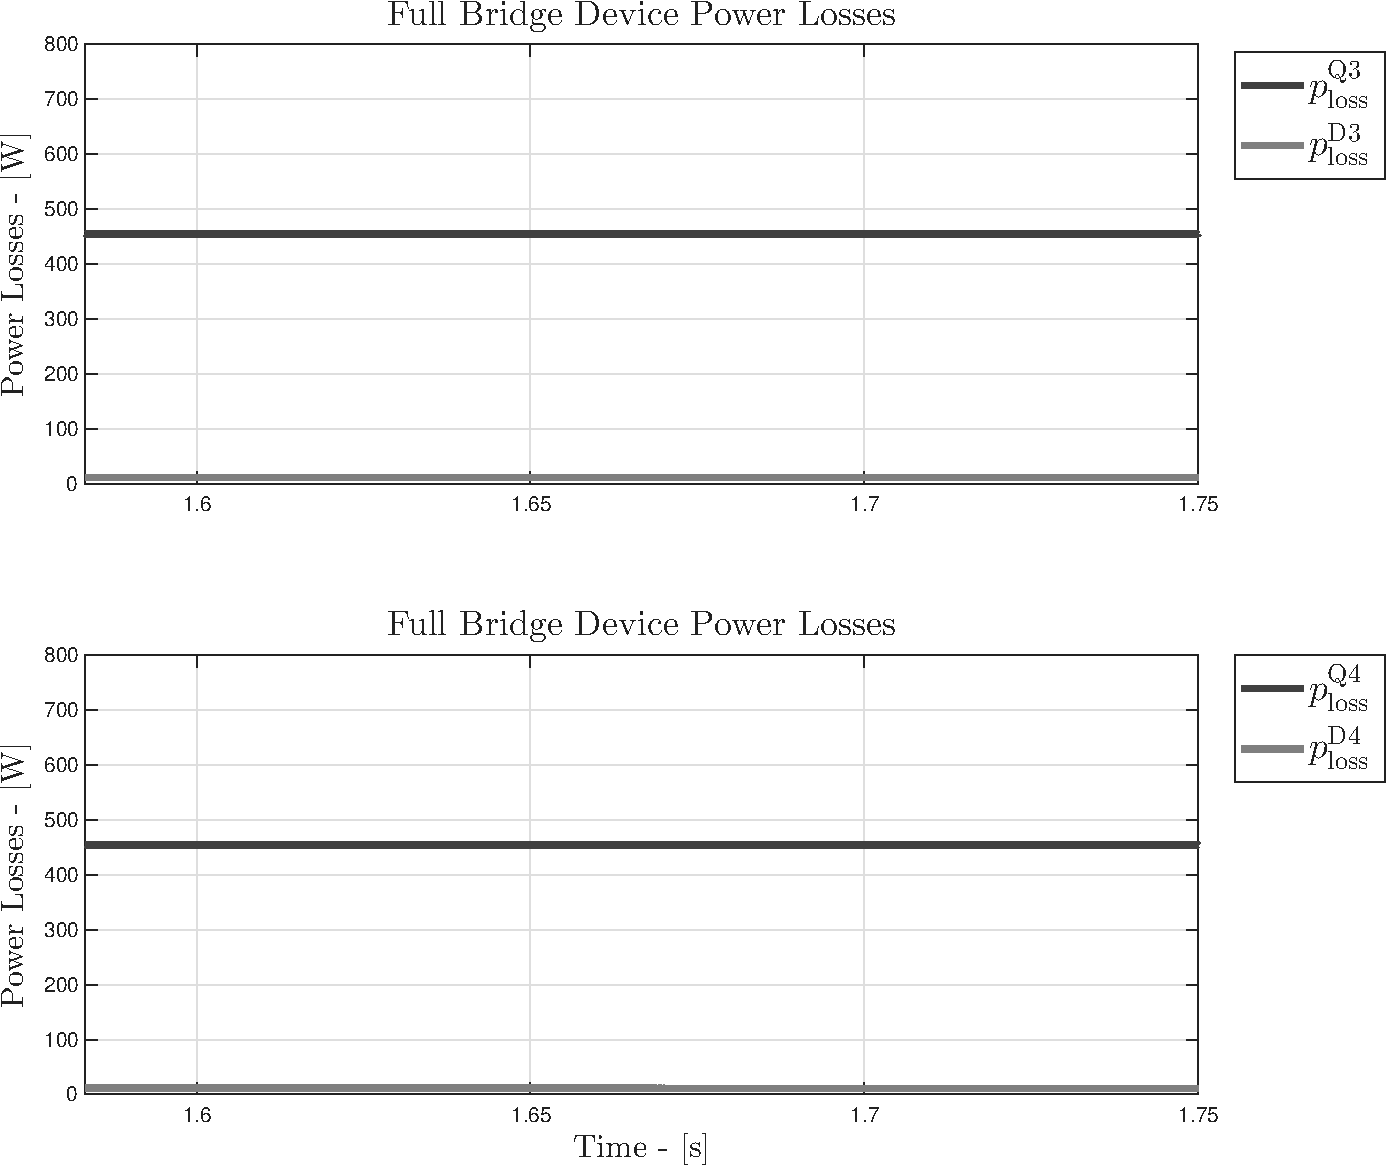
\includegraphics[width = 225pt, angle = 0, 
		keepaspectratio]{figures/sim_results_7/full_bridge_devices_power_losses_2.pdf}
		\captionsetup{width=0.75\textwidth, font=footnotesize}	
		\caption{Full Bridge device power losses (top), and (bottom).}
		\label{}
	\end{subfigure}
	\captionsetup{width=0.65\textwidth, font=small}	
	\caption{Full bridge device power losses - case scenario NLC.}
	\label{}
\end{figure}


\subsection{Case scenario NLH}
This subsection presents the simulation results for the NLH case. The simulations report the voltages and currents of the main passive and active components, as well as the corresponding losses.
\begin{figure}[H]
	\centering
	\begin{subfigure}{0.5\textwidth}
		\centering
		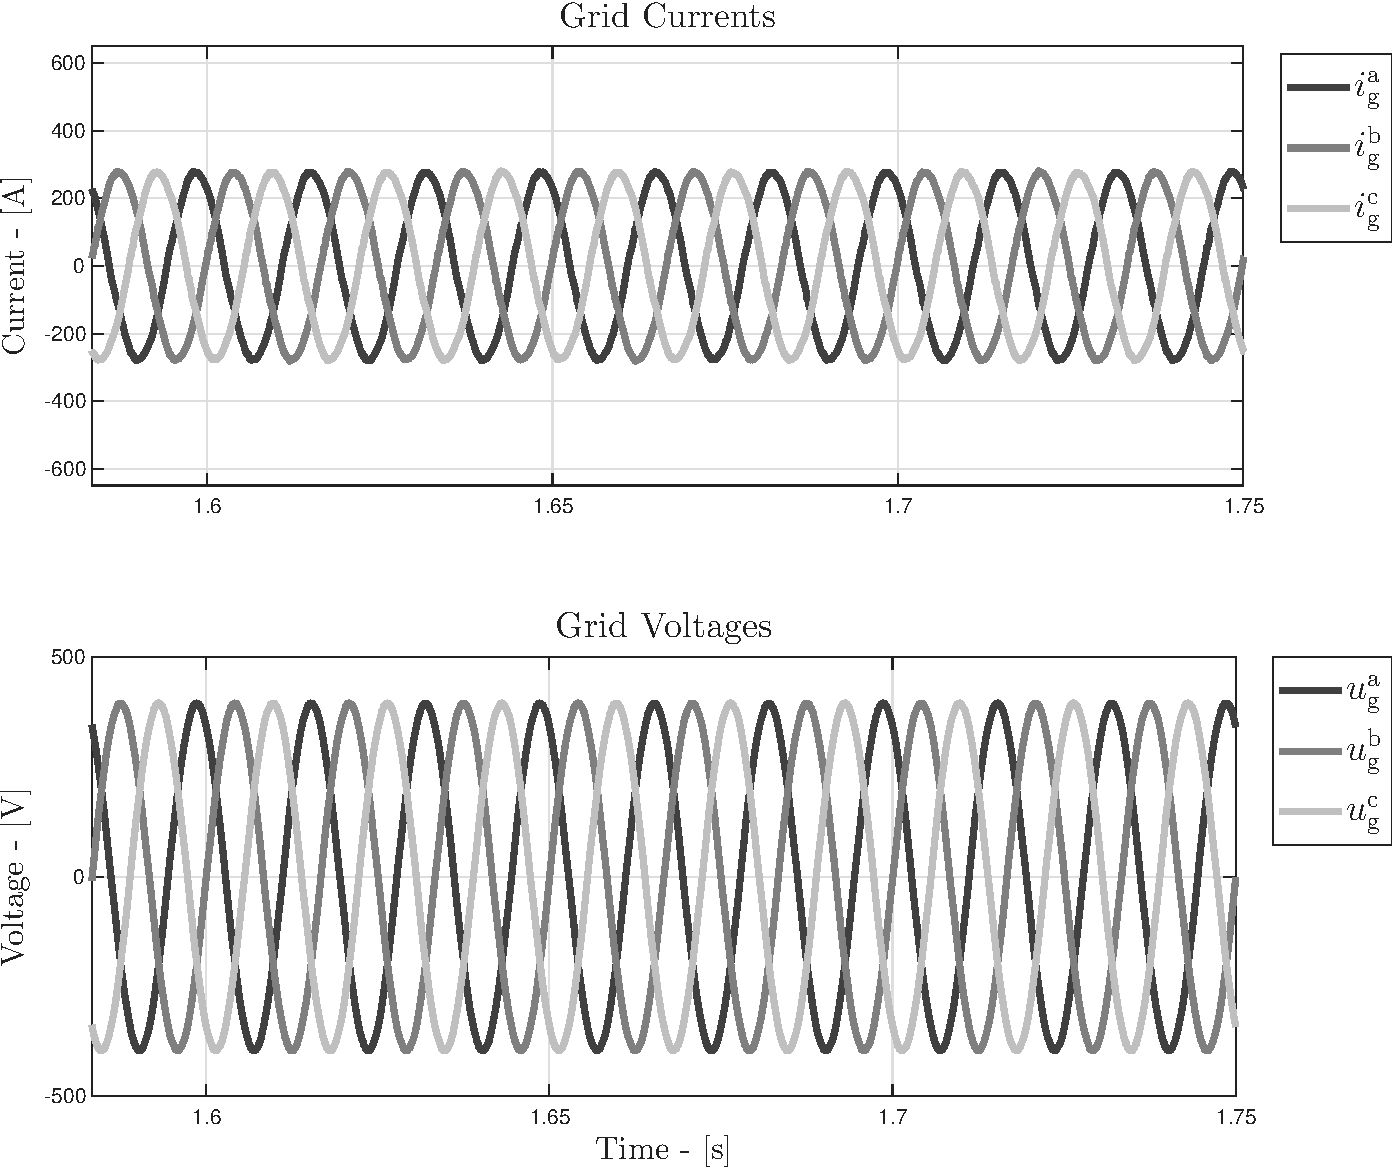
\includegraphics[width =225pt, angle = 0, 
		keepaspectratio]{figures/sim_results_8/grid_quantities.pdf}
		\captionsetup{width=0.95\textwidth, font=footnotesize}	
		\caption{Grid current waveform (top), and grid voltage waveform (bottom).}
		\label{}
	\end{subfigure}%
	\begin{subfigure}{0.5\textwidth}
		\centering
		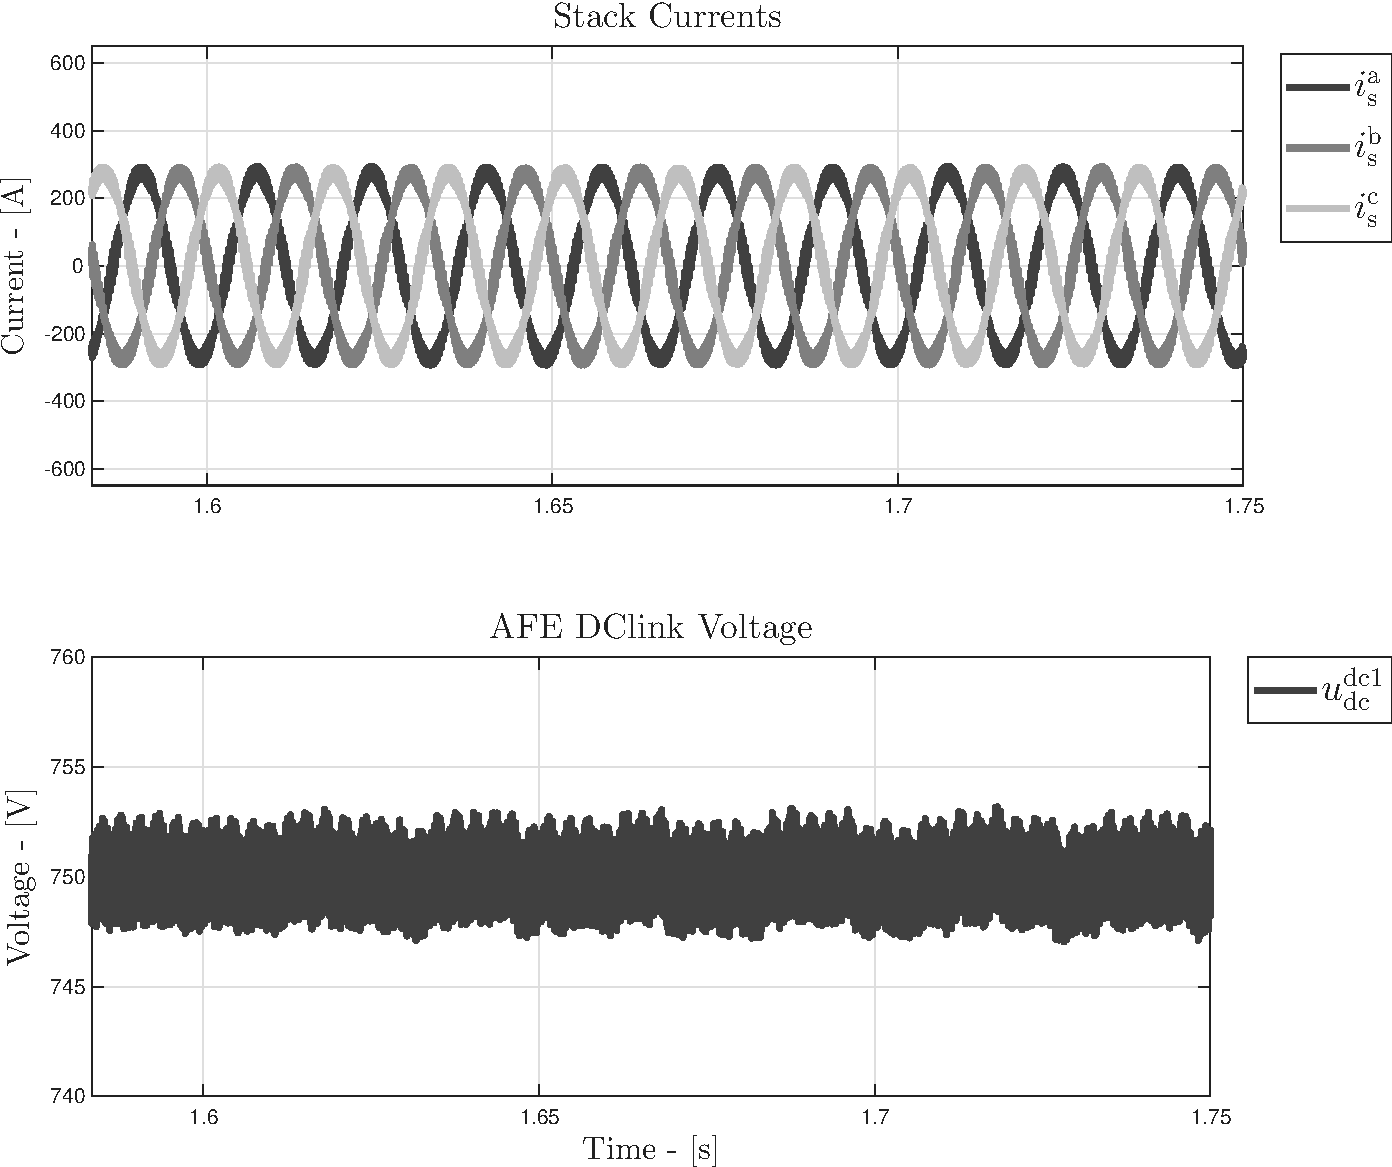
\includegraphics[width =225pt, angle = 0, 
		keepaspectratio]{figures/sim_results_8/afe_stack_quantities.pdf}
		\captionsetup{width=0.75\textwidth, font=footnotesize}	
		\caption{AFE-Stack current waveform (top), and AFE-DClink Voltage waveform (bottom).}
		\label{}
	\end{subfigure}
	\captionsetup{width=0.65\textwidth, font=small}	
	\caption{Grid and AFE stack quantities - case scenario NLH.}
	\label{}
\end{figure}

\begin{figure}[H]
	\centering
	\begin{subfigure}{0.5\textwidth}
		\centering
		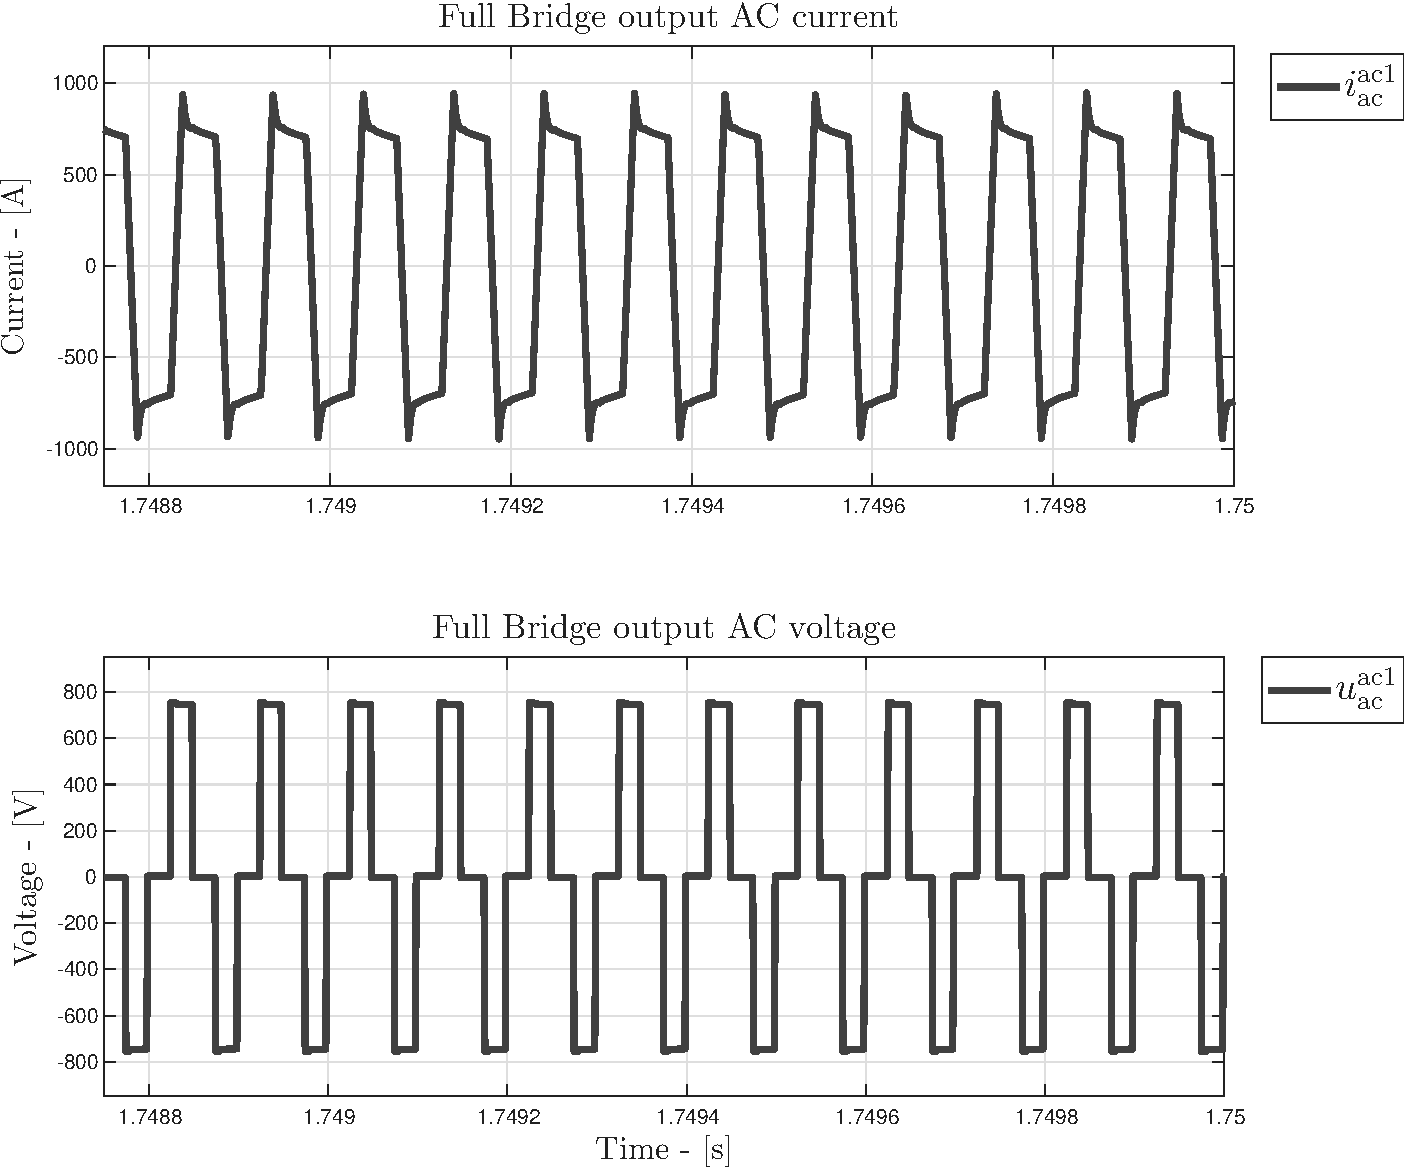
\includegraphics[width = 225pt, angle = 0, 
		keepaspectratio]{figures/sim_results_8/fbc_quantities_1.pdf}
		\captionsetup{width=0.95\textwidth, font=footnotesize}	
		\caption{Full Bridge output current (top), and output voltage (bottom).}
		\label{}
	\end{subfigure}%
	\begin{subfigure}{0.5\textwidth}
		\centering
		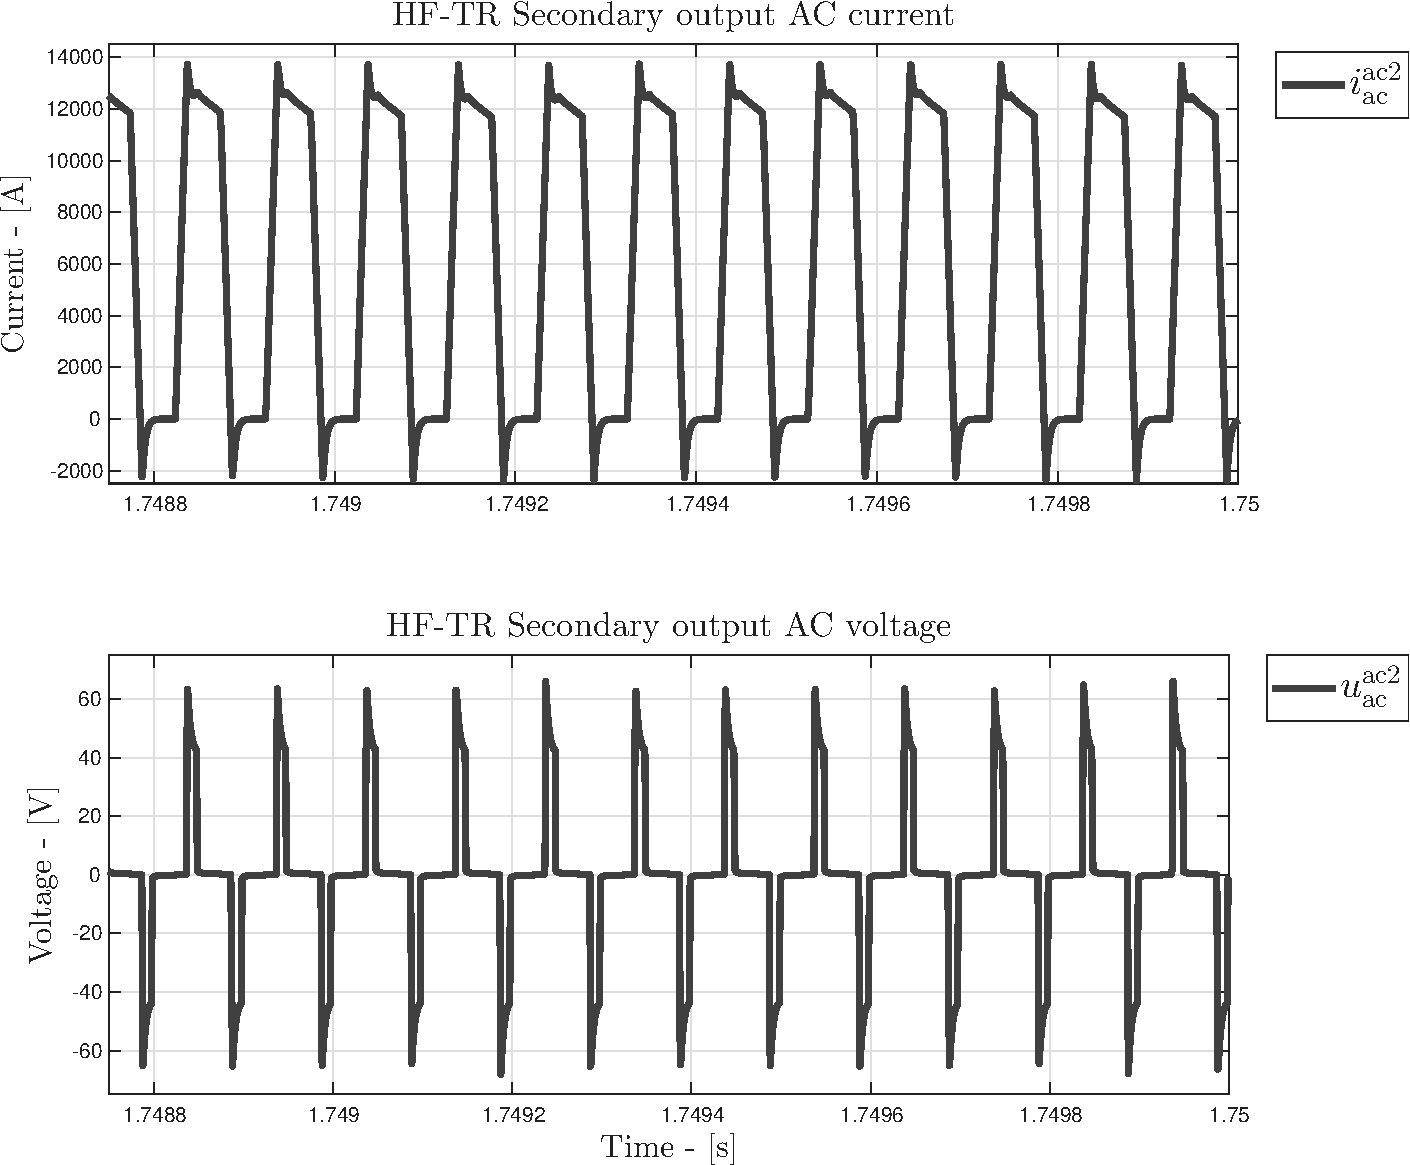
\includegraphics[width = 225pt, angle = 0, 
		keepaspectratio]{figures/sim_results_8/fbc_quantities_2.pdf}
		\captionsetup{width=0.75\textwidth, font=footnotesize}	
		\caption{HF-TR secondary current (top), and voltage (bottom).}
		\label{}
	\end{subfigure}
	\captionsetup{width=0.65\textwidth, font=small}	
	\caption{Full Bridge Converter quantities - case scenario NLH.}
	\label{}
\end{figure}

\begin{figure}[H]
	\centering
	\begin{subfigure}{0.5\textwidth}
		\centering
		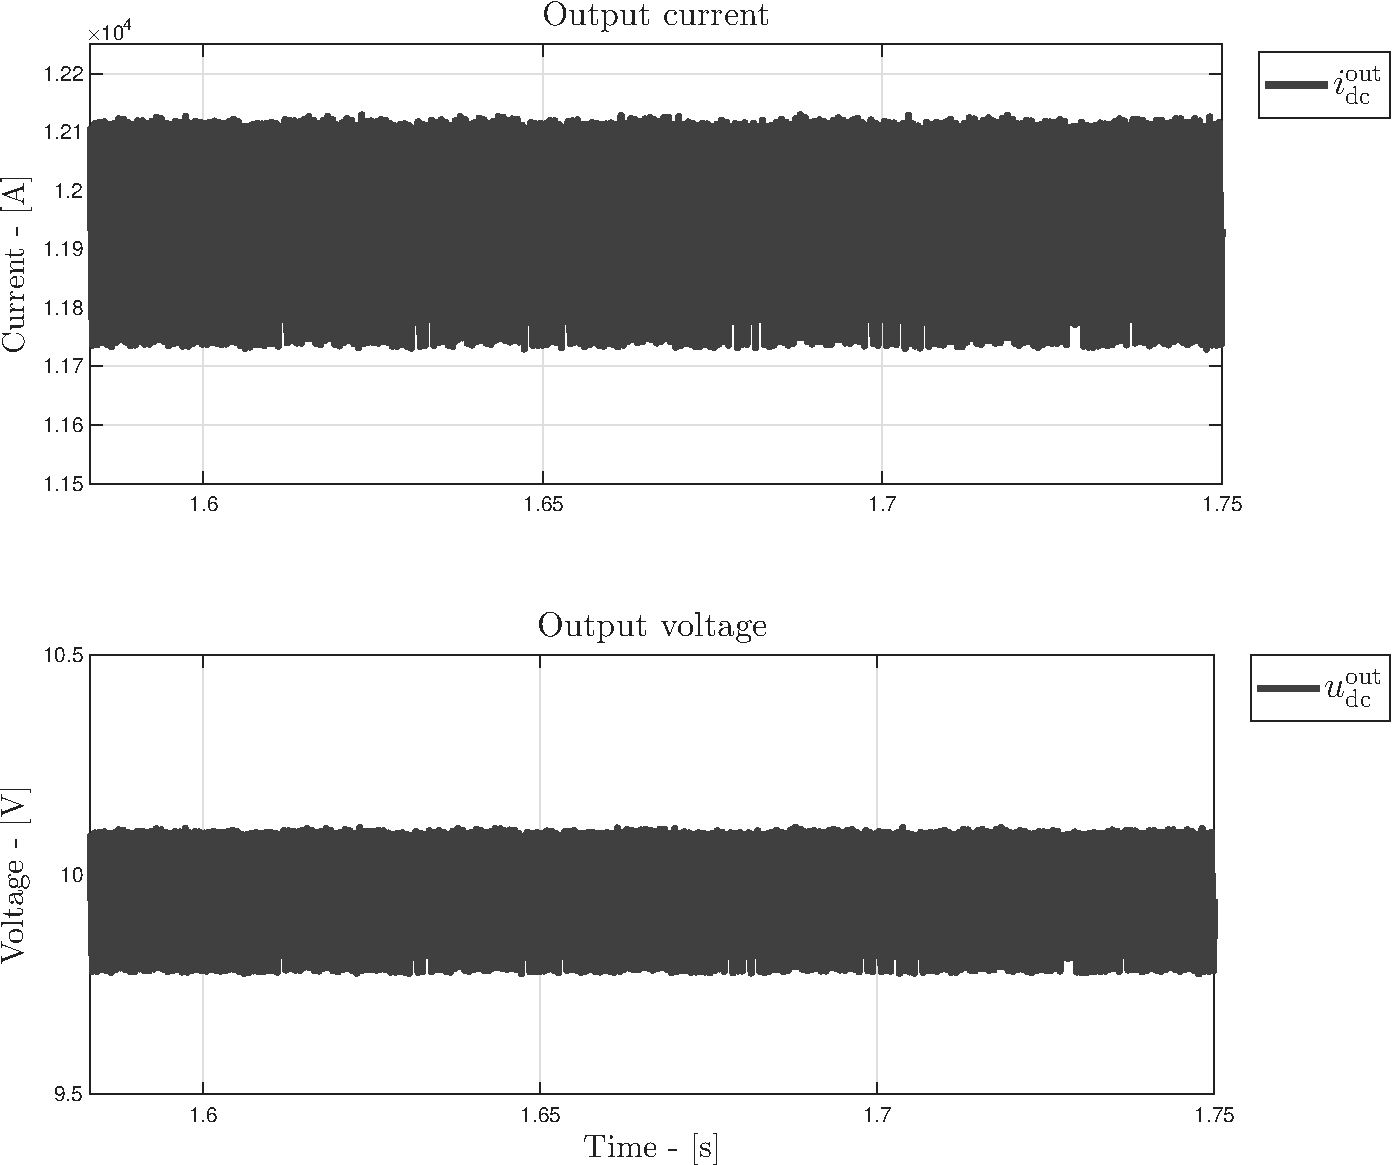
\includegraphics[width = 225pt, angle = 0, 
		keepaspectratio]{figures/sim_results_8/output_quantities.pdf}
		\captionsetup{width=0.5\textwidth, font=footnotesize}	
		\caption{Output current (top), and output voltage (bottom).}
		\label{}
	\end{subfigure}%
	\begin{subfigure}{0.5\textwidth}
		\centering
		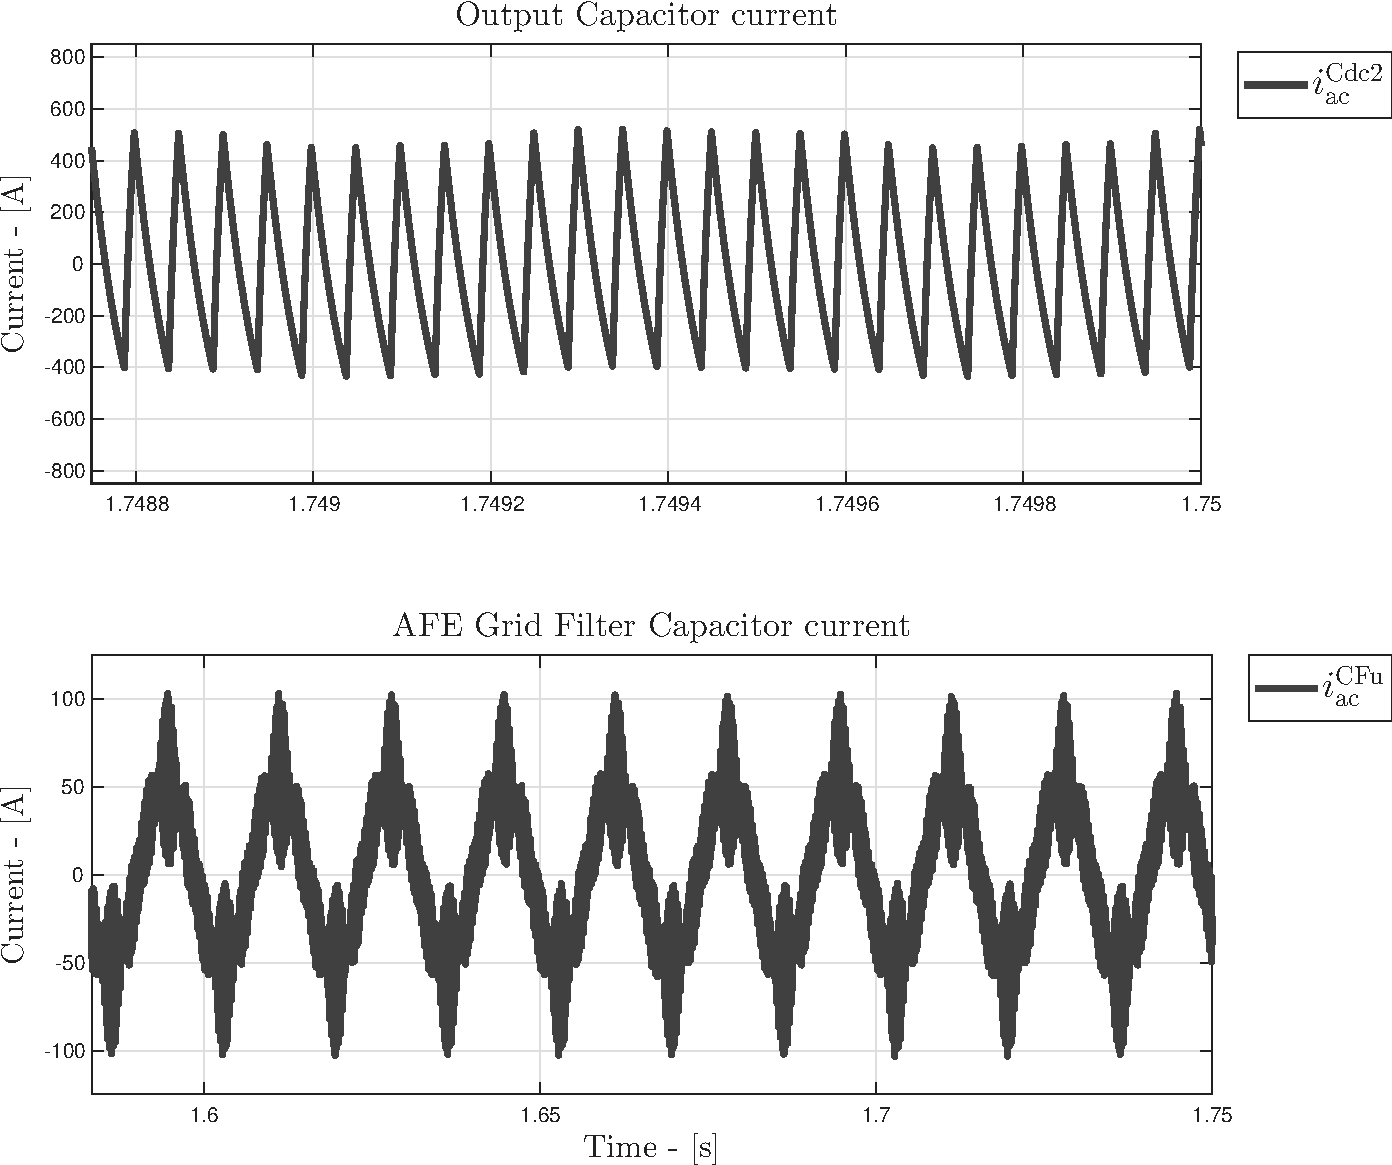
\includegraphics[width = 225pt, angle = 0, 
		keepaspectratio]{figures/sim_results_8/capacitors_currents.pdf}
		\captionsetup{width=0.95\textwidth, font=footnotesize}	
		\caption{Output filter capacitor current (top), and AFE grid filter capacitor current (bottom).}
		\label{}
	\end{subfigure}
	\captionsetup{width=0.65\textwidth, font=small}	
	\caption{Output quantities and capacitor filter currents - case scenario NLH.}
	\label{}
\end{figure}

\begin{figure}[H]
	\centering
	\begin{subfigure}{0.5\textwidth}
		\centering
		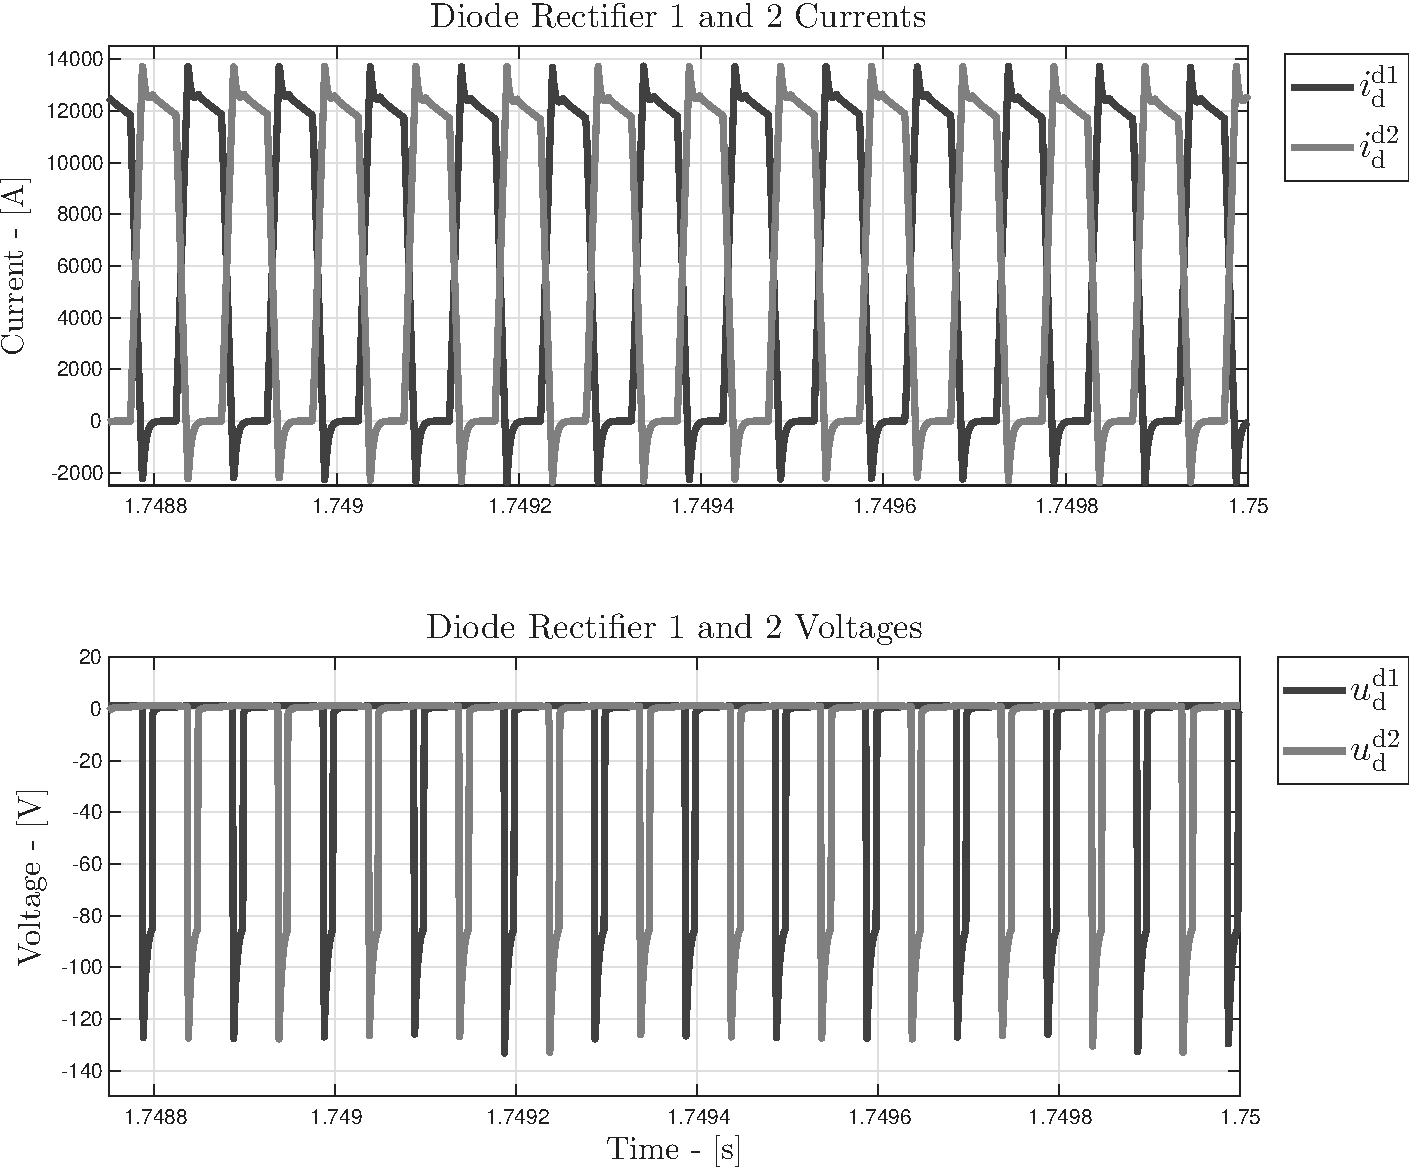
\includegraphics[width = 225pt, angle = 0, 
		keepaspectratio]{figures/sim_results_8/diode_rectifier.pdf}
		\captionsetup{width=0.75\textwidth, font=footnotesize}	
		\caption{Diode rectifier current (top), and (bottom).}
		\label{}
	\end{subfigure}%
	\begin{subfigure}{0.5\textwidth}
		\centering
		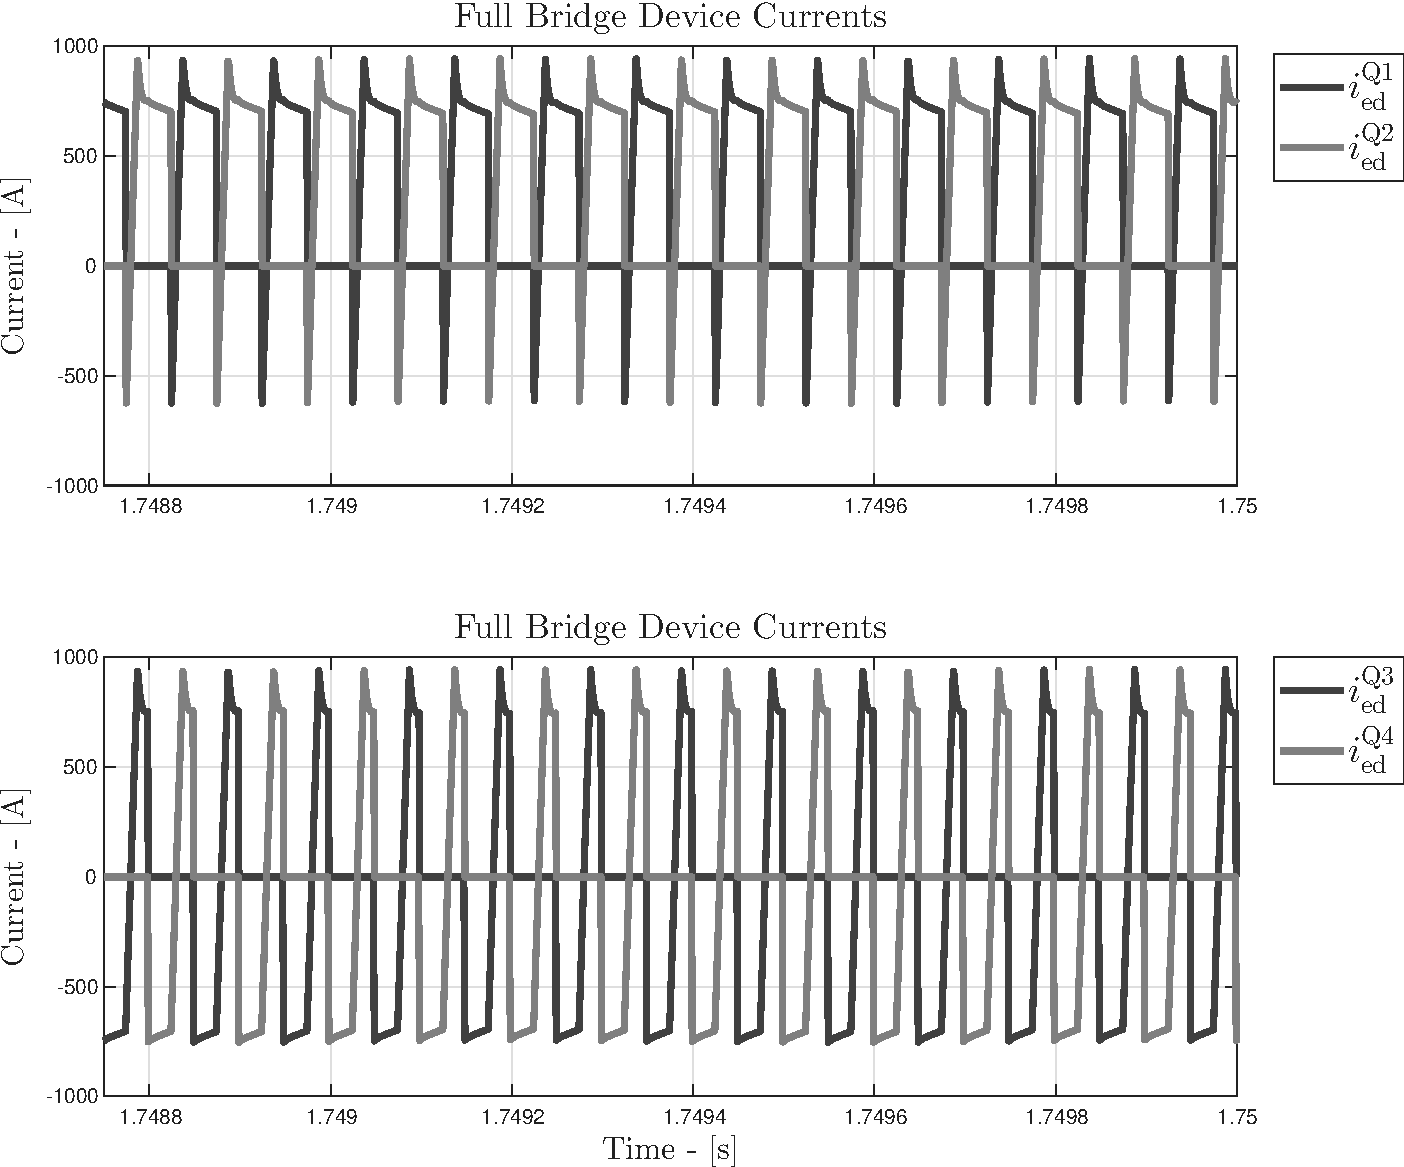
\includegraphics[width = 225pt, angle = 0, 
		keepaspectratio]{figures/sim_results_8/full_bridge_devices_quantities.pdf}
		\captionsetup{width=0.75\textwidth, font=footnotesize}	
		\caption{Full Bridge devices current (top), and (bottom).}
		\label{}
	\end{subfigure}
	\captionsetup{width=0.65\textwidth, font=small}	
	\caption{Full bridge devices current and diode rectifiers current - case scenario NLH.}
	\label{}
\end{figure}

\begin{figure}[H]
	\centering
	\begin{subfigure}{0.5\textwidth}
		\centering
		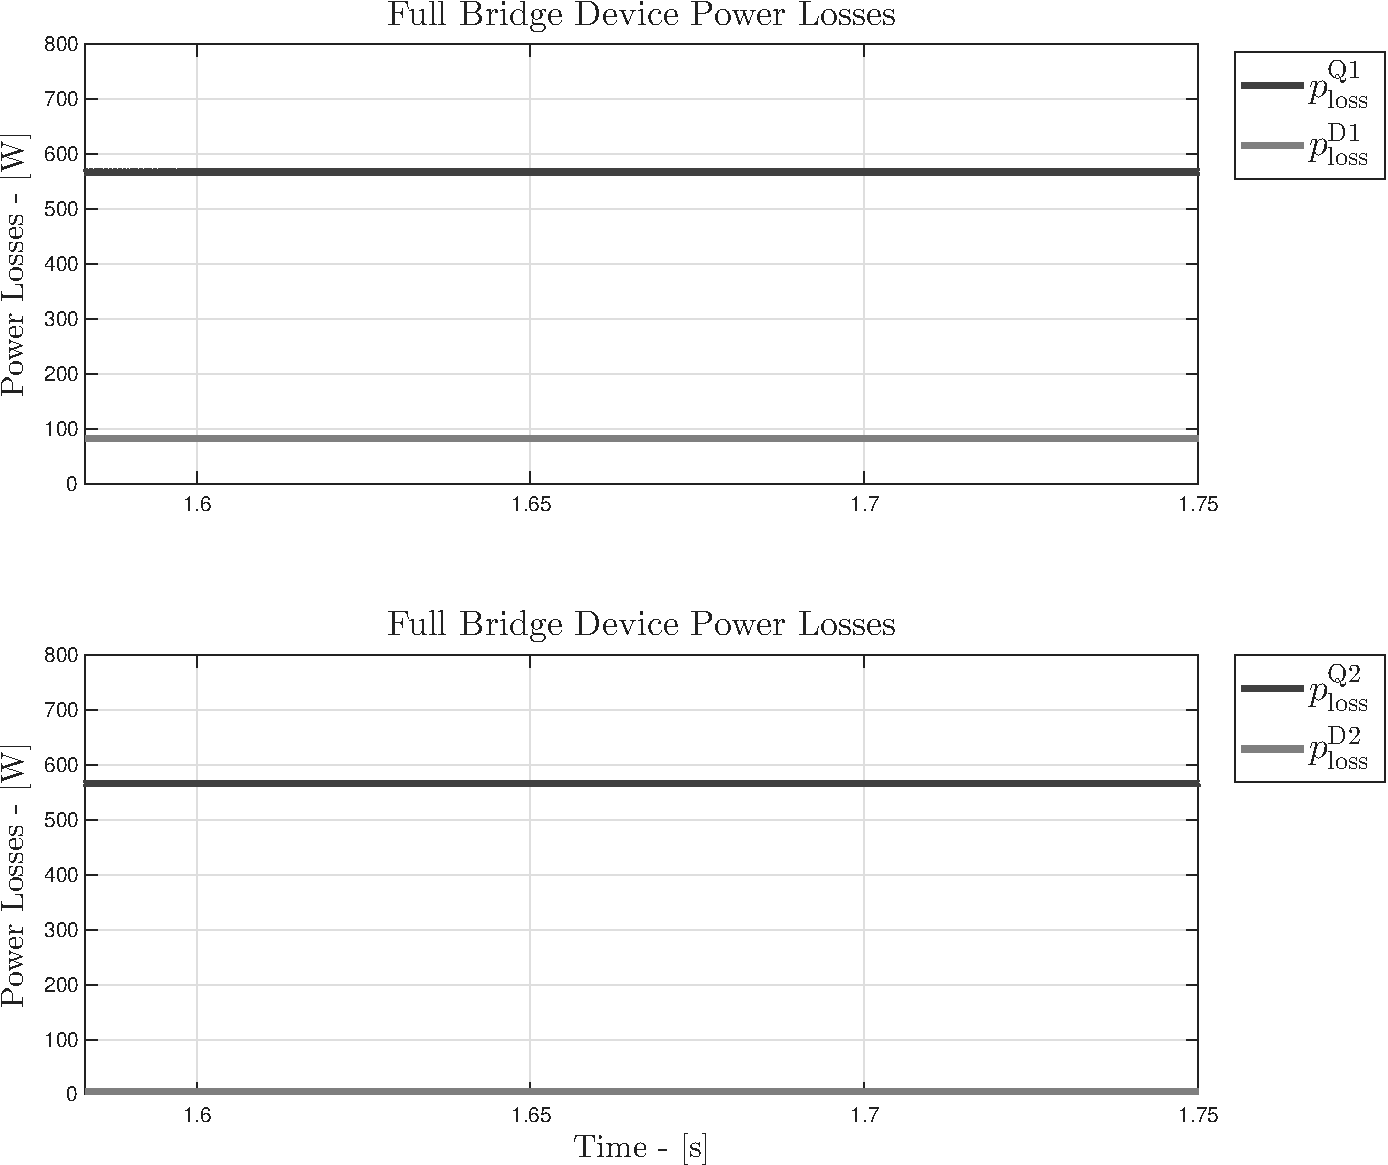
\includegraphics[width = 225pt, angle = 0, 
		keepaspectratio]{figures/sim_results_8/full_bridge_devices_power_losses_1.pdf}
		\captionsetup{width=0.75\textwidth, font=footnotesize}	
		\caption{Full Bridge device power losses (top), and (bottom).}
		\label{}
	\end{subfigure}%
	\begin{subfigure}{0.5\textwidth}
		\centering
		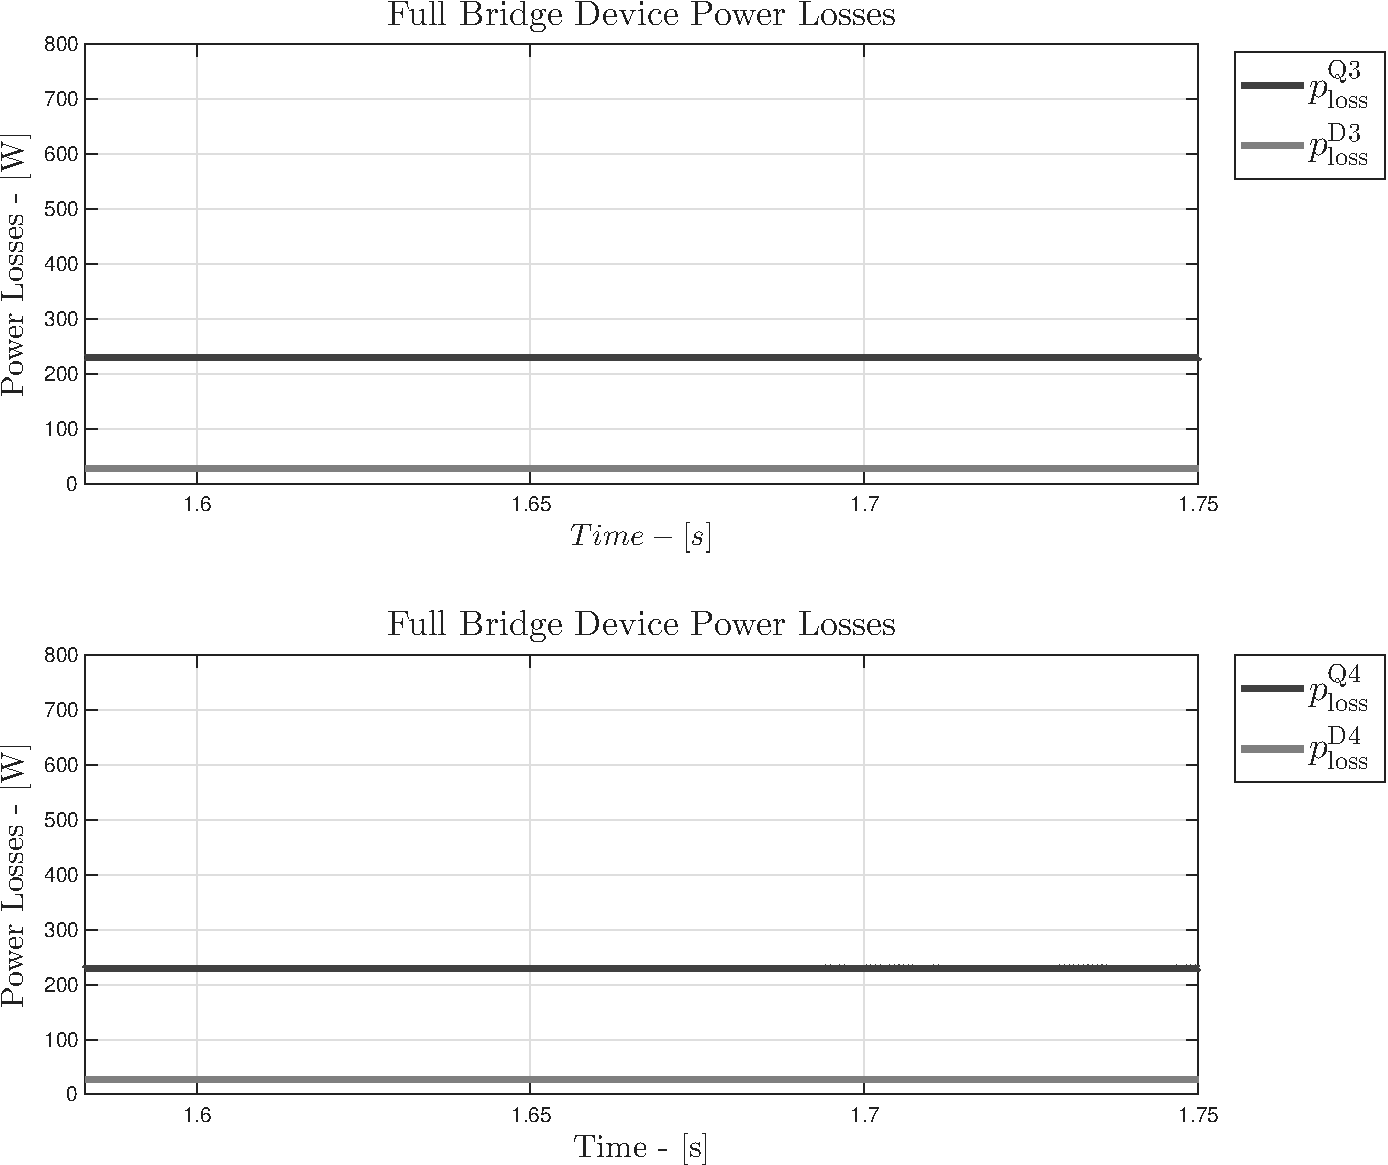
\includegraphics[width = 225pt, angle = 0, 
		keepaspectratio]{figures/sim_results_8/full_bridge_devices_power_losses_2.pdf}
		\captionsetup{width=0.75\textwidth, font=footnotesize}	
		\caption{Full Bridge device power losses (top), and (bottom).}
		\label{}
	\end{subfigure}
	\captionsetup{width=0.65\textwidth, font=small}	
	\caption{Full bridge device power losses - case scenario NLH.}
	\label{}
\end{figure}


%\begin{thebibliography}{99}
%	% power electronics
%	\bibitem{liserre} 
%	R. Teodorescu, M. Liserre, P. Rodrıguez, \emph{Grid converters for photovoltaic and wind power systems}. Wiley, 2011.
%\end{thebibliography}

\end{onehalfspace}
\end{document} 